\chapter{Analysis of .NET ORM frameworks}
\label{chapter:ormcomparison}

The chapter begins by exploring what \acrshort{orm} frameworks are, introducing core concepts in relation to the .NET framework. Modern trends and available \acrshort{orm}(s) are then reviewed, followed by the selection of a representative sample. The chosen candidates are analyzed in terms of their features, strengths, and limitations. Once a solid theoretical foundation is established, practical capabilities are verified and performance benchmarks are prepared using a set of pre-selected queries. This knowledge serves as the basis for designing translation between different \acrshort{orm}(s) in the subsequent chapters.

\section{Important concepts}
To better understand \acrshort{orm}(s) and the .NET\footnote{\url{https://dotnet.microsoft.com/en-us/}} ecosystem, important concepts have to be examined first, starting with relational data management in .NET applications. 

To request data, \acrshort{sql} query must be composed, executed through an open database connection, and results must be manually parsed. This can be achieved with the help of the standard .NET library, particularly ADO.NET.\footnote{\url{https://learn.microsoft.com/en-gb/dotnet/framework/data/adonet/}} However, by directly using \acrshort{sql} in raw strings, dependencies on a query language that lacks static typing in the context of C\# are introduced. Based on our observations, this can potentially lead to additional complexity. Nevertheless, ADO.NET remains crucial, and most .NET applications have it as a hidden dependency. All of the \acrshort{orm} frameworks introduced later rely on it for database communication. 

To lower complexity related to database communication and data persistence, abstraction provided by \acrshort{orm}(s) is used. The level of abstraction varies depending on the specific framework. There are generally two categories, micro and macro \acrshort{orm}(s)~\cite{shapovalov2024micro}. On one end of the spectrum, there are lightweight, usually performance-oriented frameworks. They offer a narrow set of features, some simple abstraction over ADO.NET. Some of those might not even be full \acrshort{orm}(s), omitting the ``relational'' part entirely~\cite{Dapper}. On the opposite end appear full-fledged frameworks that completely abstract away database communication, providing abstraction over \acrshort{sql} in the form of different query languages and an extensive set of features to simplify the work of developers.

\subsection{ADO.NET}
ADO.NET\footnote{\url{https://learn.microsoft.com/en-us/dotnet/framework/data/adonet/ado-net-overview}} provides access to different data sources, not limited to only databases. It provides components and models for connecting to the sources, executing commands, and retrieving results. All this functionality is built into \texttt{System.Data} library.

\begin{example}
\small
A shortened example from Microsoft documentation\footnote{\url{https://learn.microsoft.com/en-us/dotnet/framework/data/adonet/ado-net-overview}} demonstrates the usage of key ADO.NET objects, namely \texttt{SqlConnection}, \texttt{SqlCommand} and \texttt{SqlDataReader}. Managing the connection, building the query command, and reading results introduces a fair amount of overhead and manual control. The indexed access to \texttt{SqlDataReader} inside the \texttt{while} loop can end up being error-prone and increase the risk of runtime exceptions. Although this approach is functional, it highlights why an abstraction would be more desirable.
\qed

\begin{lstlisting}[language=CSharp]
const string connectionString = "...";

const string queryString =
    "SELECT ProductID, UnitPrice, ProductName from dbo.products "
    + "WHERE UnitPrice > @pricePoint "
    + "ORDER BY UnitPrice DESC;";

const int paramValue = 5;

using (SqlConnection connection = new(connectionString))
{
    SqlCommand command = new(queryString, connection);
    command.Parameters.AddWithValue("@pricePoint", paramValue);

    connection.Open();
    SqlDataReader reader = command.ExecuteReader();
    while (reader.Read())
    {
        Console.WriteLine($"{reader[0]}\t{reader[1]} ...");
    }
    reader.Close();
}
\end{lstlisting}
\end{example}

\subsection{Entities and mapping}
Entities are a set of classes either mirroring database tables or reflecting a domain model. Entities should be plain old \acrshort{clr} objects (\acrshort{poco}(s)). The term is derived from plain old Java objects (\acrshort{pojo}(s)). It refers to classes that do not inherit from any base class or interface. And they are not dependent on any library~\cite{Fowler2003POJO}.

\begin{example}
\small
An example of a purchase order class demonstrates a composition of \acrshort{poco}. It contains a set of properties with basic .NET data types. It has no dependencies and can be used within any framework. This entity contains no rules for mapping. It would work only with a query whose result columns match the entity properties. And of course, data types and nullability would have to match as well.
\qed
\begin{lstlisting}[language=CSharp]
class PurchaseOrder
{
    int PurchaseOrderID { get; set; }
    int SupplierID { get; set; }
    DateTime OrderDate { get; set; }
    DateTime? ExpectedDeliveryDate { get; set; }
    string? Comments { get; set; }
}
\end{lstlisting}
\end{example}

Micro \acrshort{orm}(s) do not usually use any entity mapping. They simply load resulting records into entities that match projected columns. Frameworks performing more complex non-read operations require further configuration to avoid mismatches. In some use cases, such as domain-driven development, entities might be initially designed in an application and then the corresponding schema generated with the help of some tool~\cite{FowlerDDD}.

Entity mapping might be done in multiple ways. The simplest form is inferred mapping or global conventions. The framework guesses, e.g., table and column names, data types, and nullability from entity declaration or global rules. An example of such a framework is Entity Framework Core\footnote{\url{https://learn.microsoft.com/en-us/ef/core/modeling/}}, which, without any mapping, uses default conventions to infer the mapping. Clearly, inferred mapping lacks constraints including concrete data types, numeric precision, or encoding. Those details can be specified by property and class attributes. Coupling the mapping with the entity makes it framework-dependent, which can be problematic if the domain model is meant to remain isolated from database access to avoid abstraction leakage. Mapping through code or a configuration file allows separation and is usually more expressive and powerful.

\begin{example}
\small
Let us consider two different mapping approaches and compare them. In the first instance, \texttt{PurchaseOrder} entity is mapped in Entity Framework Core\footnote{\url{https://learn.microsoft.com/en-gb/ef/core/}} using attributes and the rest of the mapping is inferred. For example, \texttt{OrderDate} will likely be mapped to a \texttt{DATETIME2} column type, with default precision. Of course, the inference is optional and more configuration attributes or mapping by code can be added to avoid any uncertainties. 
\begin{lstlisting}[language=CSharp]
[Table("PurchaseOrders", Schema = "Purchasing")]
class PurchaseOrder
{
    [Key]
    int PurchaseOrderID { get; set; }

    int SupplierID { get; set; }

    DateTime OrderDate { get; set; }
}
\end{lstlisting}
The second mapping is in the form of \acrshort{xml} mapping file using NHibernate \acrshort{orm}\footnote{\url{https://nhibernate.info/}}. This assumes a corresponding \acrshort{poco} is somewhere else in the project. This configuration is more verbose and requires more information, but prevents any issues with inference. The mapping isolation from the entity might be good for architecture, but in this case, it completely prevents automated refactoring and schema change reflection.

\qed
\begin{lstlisting}[language=CSharp]
<?xml version="1.0" encoding="utf-8" ?>
<hibernate-mapping xmlns="urn:nhibernate-mapping-2.2" namespace="NHibernateEntities">
    <class name="NHibernateEntities.PurchaseOrder, NHibernateEntities" table="PurchaseOrders" schema="Purchasing">
        <id name="PurchaseOrderID" column="PurchaseOrderID" type="int">
            <generator class="identity" />
        </id>
        <property name="SupplierID" not-null="true" />
        <property name="OrderDate" not-null="true" />
    </class>
</hibernate-mapping>
\end{lstlisting}
\end{example}

Relationships are usually mapped through navigation properties. If the relationship has a single target, the navigation property is of the related entity's type. In contrast, if the relationship can target multiple entries, a collection of the related type (e.g. \texttt{List<T>}) is used instead.

\subsection{Querying}\label{sec:queries}
Relational databases generally support only \acrshort{sql} query language. Some \acrshort{orm}(s) use \acrshort{sql} directly. But relational data and queries do not translate well into a statically typed object-oriented language. That is why Language Integrated Queries (\acrshort{linq})\footnote{\url{https://learn.microsoft.com/en-us/dotnet/csharp/linq/}} were eventually introduced into C\#.\footnote{\url{https://learn.microsoft.com/en-gb/dotnet/csharp/}} They abstract the data source and can operate over relational databases as well as other sources such as \acrshort{xml} documents, object databases, or web services.

There are two ways to write \acrshort{linq} queries. The first is called \textit{declarative query syntax} and the second \textit{method syntax}. The query syntax is more \acrshort{sql}-like and should be easier to read. However, it does not syntactically fit within the C\# language, and the compiler translates it into the method syntax anyway.

\begin{example}
\small
To get an idea of how the two approaches differ, let us consider an example adapted from the documentation of \acrshort{linq}.\footnote{\url{https://learn.microsoft.com/en-us/dotnet/csharp/linq/get-started/introduction-to-linq-queries}} The two queries execute the same way and return identical results. In fact, they get translated into identical lower-level code by the compiler.

\begin{lstlisting}[language=CSharp]
int[] numbers = [ 5, 10, 8, 3, 6, 12 ];

//Query syntax:
IEnumerable<int> numQuery1 =
    from num in numbers
    where num % 2 == 0
    orderby num
    select num;

//Method syntax:
IEnumerable<int> numQuery2 = numbers
    .Where(num => num % 2 == 0)
    .OrderBy(n => n);
\end{lstlisting}
\qed
\end{example}

By applying different methods, operations like filtering, sorting, or grouping are applied on the data source. However, no part of the query is executed until iteration over the result occurs. Or until a terminal method such as \texttt{ToList}, \texttt{First}, \texttt{Single}, or \texttt{Count} is invoked. 

If the source operates on in-memory data, it should implement \texttt{IEnumerable} interface. For remote data, such as those stored in a database, \texttt{IQueryable} interface must be implemented. The source can translate the method calls into any query language. In the case of \acrshort{orm}(s), it will likely translate \acrshort{linq} method calls into \acrshort{sql} statements.\footnote{\url{https://learn.microsoft.com/en-us/dotnet/csharp/linq/get-started/introduction-to-linq-queries}}

\section{Selection process}
With the basic concepts of \acrshort{orm}(s) established, the criteria for selecting specific frameworks for evaluation can now be introduced, potential frameworks reviewed, and a representative subset ultimately selected for detailed analysis.

Important factors are popularity and community support. Those can be estimated from the number of downloads on the .NET package manager NuGet\footnote{\url{https://www.nuget.org/}} or activity on GitHub.\footnote{\url{https://github.com/}} As not all software is open source, the scope is limited to frameworks that are. As not all software is open source, the scope is limited to frameworks that are. Outdated \acrshort{orm}(s) are also excluded. To be considered, a framework must have received at least some form of update or security fix in recent years.

Support for recent .NET versions is another essential factor. The versioning history of .NET is somewhat complicated. The original implementation, .NET Framework, was Windows-only and went up to version 4.8.1. Around 2016, Microsoft performed a major rework, focusing on cross-platform implementation. With a new name .NET Core, they started again at version 1.0. After .NET Core 3.1, the "Core" naming was dropped, and versions continued as .NET 5, .NET 6 and so on. Today, developing new applications using .NET Framework is not recommended, as it only receives security patches. The current long term support version is .NET 8, while .NET 9 is a standard term support release. In this text, we refer to the legacy platform as ``.NET Framework'' and to the new one as ``.NET Core'' or simply ``.NET''.\footnote{\url{https://dotnet.microsoft.com/en-us/platform/support/policy/dotnet-core}, \url{https://dotnet.microsoft.com/en-us/learn/dotnet/what-is-dotnet-framework}}

Another version to be aware of is .NET Standard. It is a formal \acrshort{api} specification designed to unify .NET implementations. It allows libraries to be compatible with both .NET Framework and Core by targeting a common subset of \acrshort{api}(s). However, this can restrict access to newer features and optimizations.\footnote{\url{https://dotnet.microsoft.com/en-us/platform/dotnet-standard}}

This work focuses on \acrshort{orm}(s) that support Microsoft SQL Server (\acrshort{mssql}). This is not a restrictive requirement, as all major .NET \acrshort{orm}(s) provide support for \acrshort{mssql}.

The goal is to select a representative and diverse sample of \acrshort{orm} frameworks for comparison and testing. Table~\ref{tab:orm-docs} presents a selection of considered .NET \acrshort{orm} frameworks along with links to their homepages or repositories. The final selection aims to include at least two frameworks representing both micro and macro \acrshort{orm} types, as well as frameworks that offer particularly notable capabilities.

\begin{table}[ht!]
\footnotesize
\def\arraystretch{1.25}
\definecolor{lightgreen}{RGB}{217, 234, 211}
\centering
\begin{tabular}{ll}
\toprule
\textbf{ORM} & \textbf{URL} \\
\midrule
\cellcolor{lightgreen}Dapper & \url{https://github.com/DapperLib/Dapper} \\
\cellcolor{lightgreen}Entity Framework 6 & \url{https://learn.microsoft.com/en-us/ef/ef6/} \\
\cellcolor{lightgreen}Entity Framework Core & \url{https://learn.microsoft.com/en-us/ef/core/} \\
\cellcolor{lightgreen}LINQ to DB (linq2db) & \url{https://linq2db.github.io/} \\
Massive & \url{https://github.com/FransBouma/Massive} \\
Mighty & \url{https://github.com/MightyOrm/Mighty} \\
\cellcolor{lightgreen}NHibernate & \url{https://nhibernate.info/} \\
Norm.NET & \url{https://vb-consulting.github.io/norm.net/} \\
\cellcolor{lightgreen}PetaPoco & \url{https://github.com/CollaboratingPlatypus/PetaPoco} \\
\cellcolor{lightgreen}RepoDB & \url{https://repodb.net/} \\
SqlMarshal & \url{https://github.com/kant2002/SqlMarshal} \\
XPO & \url{https://devexpress.com/Products/NET/ORM/} \\
\bottomrule
\end{tabular}
\caption{Considered ORMs with selected ones highlighted in green\label{tab:orm-docs}}
\end{table}

From the list of \acrshort{orm} frameworks, XPO was not considered due to not being open source. The other excluded frameworks were found to be outdated or inactive. This was primarily determined by the lack of recent GitHub commits and low community engagement, such as star count. 

The final selection (highlighted in light green) includes seven \acrshort{orm}(s).\textbf{Dapper}, \textbf{NHibernate}, and \textbf{Entity Framework Core} are chosen as the most widely used options. \textbf{Entity Framework 6} is included for completeness -- despite being older, it remains widely spread among legacy projects and meaningfully differs from \acrshort{ef} Core, particularly in terms of version compatibility. \textbf{PetaPoco} is selected to contrast Dapper in the micro category. During the research process, frameworks that fall between micro and macro categories were also identified, offering some abstraction without the full complexity of macro \acrshort{orm}s. \textbf{LINQ to DB} extensively supports \acrshort{linq} but stays lightweight. \textbf{RepoDB} is included based on its claim of being the ``easiest-to-use''~\cite{RepoDB}. Each \acrshort{orm} is examined in detail in the following section.

\section{Feature comparison}
The process begins by gathering sources for each \acrshort{orm}, including links to documentation, repositories, and package managers. Each framework is briefly introduced, primarily based on claims made in its official documentation. This is followed by an overview of distribution channels, licensing, and versioning information. To assess relevancy, development activity, community engagement, and available tool support are reviewed. The focus then shifts to more technical aspects, such as supported database systems and configuration options, as well as how each \acrshort{orm} handles entity and relationship mapping and various aspects of database operations.

In the context of the .NET ecosystem, the focus is placed on supported versions. Therefore, only versions explicitly targeted by the package are listed. However, as previously discussed, .NET packages typically maintain both backward and forward compatibility, and the use of .NET Standard enables targeting both .NET Framework and .NET Core.

To help assess usage, download counts are considered. These figures are obtained from the respective NuGet package pages, with aggregate counts sourced from the NuGet Trends website.\footnote{\url{https://nugettrends.com/}} Yearly downloads reflect the period between 30th June 2024 and 29th June 2025.

\subsection{Dapper}
\label{sec:feat_dapper}

Dapper~\cite{Dapper,DapperRepo} is an open-source micro \acrshort{orm} framework, originally developed by the team at Stack Overflow. It was created in response to the inefficiencies observed with LINQ to SQL, a predecessor of the Entity Framework (\acrshort{ef}), particularly under increasing traffic loads. Designed for performance and simplicity, Dapper functions as a lightweight wrapper around ADO.NET,\footnote{\url{https://learn.microsoft.com/en-gb/dotnet/framework/data/adonet/}} extending the \texttt{DbConnection} object with a set of additional methods to facilitate object mapping. Its primary focus lies in mapping \acrshort{sql} query results to .NET objects, and it does not offer built-in support for modelling relationships or managing database schemas.

The core strength of Dapper lies in minimal abstraction and high execution speed. Developers retain full control over \acrshort{sql} queries, which allows precise use of \acrshort{sql} dialect features specific to a given database system. Dapper is compatible with all \acrshort{dbms}(s) supported by ADO.NET, including Microsoft SQL Server,\footnote{\url{https://www.microsoft.com/en-gb/sql-server}} Oracle,\footnote{\url{https://www.oracle.com/database/}}  PostgreSQL,\footnote{\url{https://www.postgresql.org/}} and SQLite.\footnote{\url{https://sqlite.org/}} However, it delegates schema management entirely to the developer, as it does not provide mechanisms for schema versioning or migrations. Consequently, any changes to the database schema must be manually reflected in the \acrshort{sql} queries and the corresponding C\# entities.

Entity mapping in Dapper is handled by matching the names of query result columns with the properties of a specified .NET class. Only exact name matches are recognized, and aliases or naming conventions are not supported without relying on unofficial extensions. Relationships between entities are not automatically resolved, though the framework offers helper methods that enable manual mapping of joined queries using lambda expressions. This process still entails a non-negligible performance overhead and potential duplication, making it a practical but suboptimal alternative to proper relationship management. Moreover, Dapper does not support collection mapping or advanced data format serialization such as \acrshort{json} or \acrshort{xml}, unless the underlying \acrshort{sql} engine supports it natively and the developer writes custom \acrshort{sql} logic to handle it.

\begin{example}
\small
This code example from the Dapper repository\footnote{\url{https://github.com/DapperLib/Dapper?tab=readme-ov-file\#execute-a-query-and-map-it-to-a-list-of-typed-objects}} showcases an entity and a query returning one instance. Properties are matched and filled by name, the rest remain empty.
\qed

\begin{lstlisting}[language=CSharp]
public class Dog
{
    public int? Age { get; set; }
    public Guid Id { get; set; }
    public string Name { get; set; }
    public float? Weight { get; set; }

    public int IgnoredProperty { get { return 1; } }
}

var guid = Guid.NewGuid();
var dog = connection.Query<Dog>("select Age = @Age, Id = @Id", new { Age = (int?)null, Id = guid });
\end{lstlisting}
\end{example}

\begin{example}
\small
In this example from the same repository\footnote{\url{https://github.com/DapperLib/Dapper?tab=readme-ov-file\#multi-mapping}}, each post is connected to its owner. The lambda function in \texttt{Query} methods specifies how to connect the entities. Users are likely duplicated for each post. Overall, this is just a simplification of the manual handling of the data, and overhead is still present. Real use cases could be more complex and inefficient.
\qed

\begin{lstlisting}[language=CSharp]
var sql =
@"select * from #Posts p
left join #Users u on u.Id = p.OwnerId
Order by p.Id";

var data = connection.Query<Post, User, Post>(
    sql, (post, user) => { post.Owner = user; return post;});
var post = data.First();
\end{lstlisting}
\end{example}

Dapper does not include capabilities such as change tracking, data seeding, or query logging. Batch operations are supported natively, while bulk operations require the use of a commercial extension (Dapper Plus).\footnote{\url{https://dapper-plus.net/}} Transaction handling is available indirectly through ADO.NET or via community-supported extensions. All major methods have asynchronous counterparts, ensuring compatibility with modern asynchronous programming models in .NET. Despite the lack of official development tools, Dapper benefits from a variety of extensions, both official and community-driven. Notable examples include \texttt{Dapper.SqlBuilder}\footnote{\url{https://github.com/DapperLib/Dapper/tree/main/Dapper.SqlBuilder}} for SQL generation, \texttt{Dapper.Rainbow}\footnote{\url{https://github.com/DapperLib/Dapper/tree/main/Dapper.Rainbow}} for simplified CRUD operations, and \texttt{Dapper.EntityFramework}\footnote{\url{https://github.com/DapperLib/Dapper/tree/main/Dapper.EntityFramework}} for integrating with Entity Framework -- although the latter remains largely undocumented.

The project is distributed under the Apache 2.0 License\footnote{\url{https://github.com/DapperLib/Dapper/blob/main/License.txt}} and is freely available via GitHub\footnote{\url{https://github.com/DapperLib/Dapper}} and NuGet\footnote{\url{https://www.nuget.org/packages/dapper/}}. As of the latest release (version 2.1.66 in February 2025), Dapper has amassed over 496 million total downloads, with 144 million downloads in the past year alone.\footnote{\url{https://nugettrends.com/packages?months=72&ids=Dapper}} While the release cycle is not fixed, updates follow semantic versioning and are typically introduced in response to patches or new feature demands. The framework supports multiple .NET versions, including .NET Framework, .NET Standard, and .NET~8.

In terms of community support, Dapper exhibits a healthy level of maintenance with active issue tracking and contributions. Although responses to GitHub issues may be delayed, many questions receive attention either from maintainers or the broader community, including the original authors. Documentation is primarily hosted on an external website, Learn Dapper,\footnote{\url{https://www.learndapper.com/}} which is maintained by a sponsor responsible for developing the commercial extension Dapper Plus.

\afterpage{
\begin{landscape}
\begin{table}[H]
\scriptsize
\def\arraystretch{1.45}
\centering
\caption{Comparison overview of \acrshort{orm} framework: Dapper}
\begin{tabular}{ll}
\toprule
\textbf{Property} & \textbf{Dapper} \\
\midrule
\textbf{Type} & Micro \acrshort{orm} for .NET \\
\textbf{License} & Apache 2.0 \\
\textbf{Cost} & Free; Dapper Plus is paid extension  \\
\textbf{Sources} & \url{https://github.com/DapperLib/Dapper}, \url{https://www.nuget.org/packages/Dapper}, \url{https://www.learndapper.com} \\
\textbf{Latest version} & 2.1.66 (February 2025) \\
\textbf{Supported .NET} & .NET Framework, .NET Standard, .NET 8 \\
\textbf{\acrshort{orm} features} & Object mapping only; no relationship or collection support \\
\textbf{Query support} & Raw \acrshort{sql}; any dialect via ADO.NET; no \acrshort{linq} support \\
\textbf{Mapping} & Maps result columns to entity properties by exact name; no aliases or conventions \\
\textbf{Relationship mapping} & Not supported directly; JOINs and result splitting possible manually \\
\textbf{Schema handling} & No migrations; schema defined in \acrshort{dbms}; \acrshort{sql} must be adjusted manually \\
\textbf{Change tracking} & Not supported \\
\textbf{Data seeding} & Not supported \\
\textbf{Query logging} & Not supported \\
\textbf{Transactions} & Supported via ADO.NET; extensions available \\
\textbf{Bulk operations} & Paid extension required \\
\textbf{Async support} & Fully supported \\
\textbf{Caching} & Entity mapping cached internally; no data caching \\
\textbf{Community} & Maintained actively on GitHub; many questions on Stack Overflow, often answered by the author \\
\textbf{Documentation} & External site (Learn Dapper), maintained by extension sponsor; repository includes tests and examples \\
\textbf{Extensions (official)} & Dapper.SqlBuilder, Dapper.Rainbow, Dapper.EntityFramework \\
\textbf{Extensions (community)} & Dapper Plus (paid), Dapper.Transaction \\
\textbf{Tooling} & None available \\
\textbf{Supported databases} & All ADO.NET-compatible \acrshort{dbms}(s), such as, e.g., SQL Server, Oracle, SQLite, PostgreSQL \\
\textbf{Ideal use cases} & High-performance data reading, performance bottleneck zones, apps requiring full \acrshort{sql} control \\
\bottomrule
\end{tabular}
\end{table}
\end{landscape}
}

\subsection{PetaPoco}
\label{sec:feat_petapoco}

PetaPoco~\cite{PetaPoco} is the second chosen micro \acrshort{orm}. Although it changed recently, it used to have a single-file codebase with no dependencies. It is focused on performance and simplicity. Internally it uses ADO.NET like Dapper, yet it provides its own abstractions over it. The framework is configurable through a builder, resulting in \texttt{IDatabase} interface, on which methods are called. With a focus on mapping query results to objects, it does not provide any support for relationships. It provides full control over \acrshort{sql} with an inbuilt \acrshort{sql} builder to make composing it easier. 

Its small feature set and zero dependencies enable compatibility with a wide selection of database systems, including \acrshort{mssql}, MS Access,\footnote{\url{https://support.microsoft.com/en-us/access}} SQLite, MySQL,\footnote{\url{https://www.mysql.com/}} MariaDB,\footnote{\url{https://mariadb.org/}} and Oracle. Schema management is left to the developer. Templates for entity generation out of a database schema were provided, but were deprecated in the last major version.

Entity mapping supports automatic configuration through naming conventions, such as pluralizing property names to match database columns. A limited set of mapping attributes is offered. These can be used to map table and column names, primary keys, and ignore class properties. Like Dapper, it does not automatically handle relationships but provides helper methods for manual JOINs management.

\begin{example}
\small
In the following example, the table name and primary key are explicitly defined using attributes, while other properties rely on automatic mapping. The use of the \acrshort{sql} query builder is demonstrated. The projection and source table components in the query builder can be omitted when they can be inferred from the source entity.
\qed

\begin{lstlisting}[language=CSharp]
using PetaPoco;

[TableName("Sales.OrderLines")]
[PrimaryKey("OrderLineID")]
public class OrderLine
{
    public int OrderID { get; set; }
    public int OrderLineID { get; set; }
    public decimal? UnitPrice { get; set; }
}

decimal unitPrice = 25m;
var orderLines = db.Fetch<OrderLine>(
    Sql.Builder.Where("UnitPrice = @0", unitPrice)
);
\end{lstlisting}
\end{example}

No support for advanced data formats of collections is provided, with the exception of writing native \acrshort{sql} that can work with these structures. \acrshort{linq} is not supported. Unofficial extension \texttt{StaTypPocoQueries.PetaPoco}\footnote{\url{https://github.com/asherber/StaTypPocoQueries.PetaPoco}} provides result modification methods such as \texttt{First}, \texttt{Single}, \texttt{Page}, and \texttt{Delete} with some selection capabilities. For \textit{data manipulation language} (\acrshort{dml}) operations, strongly-typed methods like \texttt{Insert}, \texttt{Save}, \texttt{Update}, and \texttt{Delete} are provided. 

Queries executed by the framework can be inspected during debugging. Transactions are supported, including nested transactions if the underlying database system allows. However, bulk operations are not available. Asynchronous versions of all methods are also provided. Advanced capabilities such as versioning, change tracking, and data seeding are not provided. The only notable extension is an unofficial \texttt{PetaPoco.SqlKata}\footnote{\url{https://github.com/asherber/PetaPoco.SqlKata}}, which is a more extensive \acrshort{sql} builder than the native one.

The library is distributed under the Apache 2.0 License\footnote{\url{https://github.com/CollaboratingPlatypus/PetaPoco/blob/development/LICENSE.txt}} and is open-sourced on GitHub\footnote{\url{https://github.com/CollaboratingPlatypus/PetaPoco}} and NuGet.\footnote{\url{https://www.nuget.org/packages/PetaPoco.Compiled/}} PetaPoco was downloaded 1.8 million times in total, with 600 thousands in the last year.\footnote{\url{https://nugettrends.com/packages?months=72&ids=PetaPoco.Compiled}} PetaPoco has been stagnating on major version 6 (6.0.683 in September 2024) for the past few years, with minor patches being done every few months in response to security patches or new feature demands. The library targets .NET Framework and Standard.

This \acrshort{orm} does not benefit from extensive community support, with the only extensive source of information being its GitHub wiki.\footnote{\url{https://github.com/CollaboratingPlatypus/PetaPoco/wiki}} Integration tests for most database systems are available and could be used for reference.

\afterpage{
\begin{landscape}
\begin{table}[H]
\scriptsize
\def\arraystretch{1.45}
\centering
\caption{Comparison overview of \acrshort{orm} framework: PetaPoco}
\begin{tabular}{ll}
\toprule
\textbf{Property} & \textbf{PetaPoco} \\
\midrule
\textbf{Type} & Micro \acrshort{orm} for .NET \\
\textbf{License} & Apache 2.0 \\
\textbf{Cost} & Free \\
\textbf{Sources} & \url{https://github.com/CollaboratingPlatypus/PetaPoco}, \url{https://www.nuget.org/packages/PetaPoco.Compiled}  \\
\textbf{Latest version} & 6.0.683 (September 2024) \\
\textbf{Supported .NET} & .NET Framework, .NET Standard \\
\textbf{\acrshort{orm} features} & Object mapping only; no relationship or collection support \\
\textbf{Query support} & Raw \acrshort{sql}; wide \acrshort{dbms} support \\
\textbf{Mapping} & Maps automatically by exact name; conventions and some attributed available \\
\textbf{Relationship mapping} & Not supported directly; JOINs and result splitting possible manually \\
\textbf{Schema handling} & No migrations; schema defined in \acrshort{dbms}; \acrshort{sql} must be adjusted manually \\
\textbf{Change tracking} & Not supported \\
\textbf{Data seeding} & Not supported \\
\textbf{Query logging} & Accessible while debugging \\
\textbf{Transactions} & Supported; with nesting \\
\textbf{Bulk operations} & Not supported \\
\textbf{Async support} & Fully supported \\
\textbf{Caching} & No caching \\
\textbf{Community} & Maintained actively on GitHub; questions and issues not frequently responded to \\
\textbf{Documentation} & GitHub wiki; repository includes integration and unit tests\\
\textbf{Extensions (official)} & None \\
\textbf{Extensions (community)} & PetaPoco.SqlKata, StaTypPocoQueries.PetaPoco \\
\textbf{Tooling} & None available \\
\textbf{Supported databases} & \acrshort{mssql}, MS Access, SQLite, MySQL, MariaDB, Oracle, etc. \\
\textbf{Ideal use cases} & High-performance data reading, performance bottleneck zones, apps requiring full \acrshort{sql} control \\
\bottomrule
\end{tabular}
\end{table}
\end{landscape}
}



\subsection{RepoDB}
RepoDB~\cite{RepoDB, RepoDBRepo} is an \acrshort{orm} for .NET bridging the gap between micro and macro \acrshort{orm}(s). It supposedly focuses on improving the developer experience, while maintaining the speed of macro \acrshort{orm}(s). It requires only a connection string and should work \textit{out of the box}. Developed by Michael Camara Pendon, it is one of the more recent libraries, starting development in 2018. It provides a set of extension methods over \texttt{Microsoft.Data.SqlClient.SqlConnection} object. 

The core package supports any database system through ADO.NET, limiting querying through raw \acrshort{sql}. To utilize strongly typed queries, database-specific extension package is required. The developer can select from \acrshort{mssql}, SQLite, MySQL, and PostgreSQL. Schema management or entity generation is not offered. Automatic entity mapping to a result can be extended using property and class attributes or a fluent mapping interface. Relationship mapping is not supported, an interface for querying multiple results at once can be utilized. Raw join \acrshort{sql} query with manual handling is another option.

\begin{example}
\small
In the example~\cite{RepoDB} below, the fluent mapping interface can be seen on a \texttt{Customer} entity. The main advantages here are separation from the entity and more programmatic configuration.
\qed

\begin{lstlisting}[language=CSharp]
FluentMapper
.Entity<Customer>()
.Table("[sales].[Customer]")
.Primary(e => e.Id)
.Column(e => e.FirstName, "[FName]")
.DbType(e => e.DateOfBirth, DbType.DateTime2);
\end{lstlisting}
\end{example}

The main focus of RepoDB is abstracting \acrshort{sql}. However, \acrshort{linq} is not supported, and queries have to be performed through one of the following options. The main interface is type-safe expressions -- for example, see the following example querying one customer by id: \lstinline{connection.Query<Customer>(e => e.Id == 25)}. The second option is \texttt{QueryField} and \texttt{QueryGroup} objects. As you can see in \lstinline{connection.Query<Customer>(new QueryField("Id", Operation.Equal, 25))}, this option is not type-safe, but should be more expressive as operator support for the first option is limited. In addition, there are more provided functions over the connection, such as \texttt{Sum}, \texttt{Max}, \texttt{Exists} functions. Data manipulation is possible using \texttt{Insert}, \texttt{Update} and \texttt{Delete} functions. Both batch and bulk operations are supported, though the latter only for \acrshort{mssql} and PostgreSQL.

Transactions are supported through ADO.NET. Application-level cache is supported in-memory, with options for custom providers. Database schema and queries are also cached, speeding up subsequent queries. The library offers a wide variety of interfaces for extension. One example can be query tracing and logging, which is provided by default but can be easily added. While the library provides asynchronous methods, there is no mention of them in the documentation. More advanced features such as change tracking, data seeding, or migration support are not provided. The \acrshort{orm} also focuses on providing the user with the implementation of common repository and unit of work patterns.

The project is open-source and distributed under Apache 2.0 license\footnote{\url{https://github.com/mikependon/RepoDB/blob/master/LICENSE.txt}} on GitHub\footnote{\url{https://github.com/mikependon/RepoDB}} and NuGet.\footnote{\url{https://www.nuget.org/packages/repodb}} With the latest version 1.13.1 released in March 2023, the updates are infrequent. The development is currently paused as per the author's comment~\cite{PendonRepoDBComment}. The project has over 1.9 million total downloads, approximately half a million of those gained in the past year.\footnote{\url{https://nugettrends.com/packages?months=72&ids=RepoDb}} .NET versions 7 and Standard are targeted. The documentation is hosted on a separate website~\cite{RepoDB}. It provides several tutorials and widely describes available classes and \acrshort{api}(s). However, it mostly reads as developer documentation; contextual explanations and longer examples are missing. Missing examples can be substituted by extensive unit and integration tests available in the repository. No extensions are provided, except those for specific database systems already discussed.


\afterpage{
\begin{landscape}
\begin{table}[H]
\scriptsize
\def\arraystretch{1.45}
\centering
\caption{Comparison overview of \acrshort{orm} framework: RepoDB}
\begin{tabular}{ll}
\toprule
\textbf{Property} & \textbf{RepoDB} \\
\midrule
\textbf{Type} & \acrshort{orm} for .NET \\
\textbf{License} & Apache 2.0 \\
\textbf{Cost} & Free \\
\textbf{Sources} & \url{https://repodb.net/}, \url{https://github.com/mikependon/RepoDB}, \url{https://www.nuget.org/packages/repodb}  \\
\textbf{Latest version} & 1.13.1  (March 2023) \\
\textbf{Supported .NET} & .NET Standard, .NET 7 \\
\textbf{\acrshort{orm} features} & Object mapping only; no relationship or collection support \\
\textbf{Query support} & Limited lambda expression support, QueryField and QueryGroup objects \\
\textbf{Mapping} & Attributes and fluent interface \\
\textbf{Relationship mapping} & Not supported directly; JOINs and result splitting possible manually \\
\textbf{Schema handling} & No migrations; schema defined in \acrshort{dbms}; queries must be adjusted manually \\
\textbf{Change tracking} & Not supported \\
\textbf{Data seeding} & Not supported \\
\textbf{Query logging} & Extensible tracing interface; must be implemented \\
\textbf{Transactions} & Supported \\
\textbf{Bulk operations} & Supported for \acrshort{mssql} and PostgreSQL \\
\textbf{Async support} & Supported, undocumented \\
\textbf{Caching} & Application-level caching \\
\textbf{Community} & Maintained on GitHub; questions and issues responded to; development currently paused \\
\textbf{Documentation} & Separate website; repository includes integration and unit tests\\
\textbf{Extensions (official)} & Database support extensions \\
\textbf{Extensions (community)} & None \\
\textbf{Tooling} & None available \\
\textbf{Supported databases} & \acrshort{mssql}, SQLite, MySQL, and PostgreSQL \\
\textbf{Ideal use cases} & Simple applications, beginner developers, performance-dependent applications possible \\
\bottomrule
\end{tabular}
\end{table}
\end{landscape}
}


\subsection{LINQ to DB}
\label{section:linqToDb}

LINQ to DB~\cite{linq2db, linq2dbRepo}, alternatively linq2db, is an \acrshort{orm} that focuses primarily on offering a type-safe layer above \acrshort{sql} through \acrshort{linq}. Statically typed, compiler-checked queries are a huge benefit for bigger projects and allow easier refactoring. It supports extensive entity and relationship mapping and should offer the best performance in terms of querying through \acrshort{linq}. Relative to that focus, it does not offer features expected from full-fledged macro \acrshort{orm}(s). There is no change tracking or caching with this framework.

LINQ to DB is compatible with a big range of database systems, e.g., \acrshort{mssql}, MySQL, Oracle, PostgreSQL, MS Access, SQLite, and even less common ones like SAP HANA,\footnote{\url{https://www.sap.com/products/data-cloud/hana/what-is-sap-hana.html}} ClickHouse,\footnote{\url{https://clickhouse.com/}}. Database schema must be handled by the developer, but entity generation from the database is available. Configuration is fairly simple through the \texttt{DataConnection} object. This object can be inherited from, allowing configuration of a wide set of options, including entity mapping. Mapping can be done using fluent methods using the aforementioned object. Another option is attributes on the entity class and properties. Convention-based and automatic mapping is also an option. All multiplicities of relationships are configurable, although the documentation provides limited information on this topic.\footnote{\url{https://linq2db.github.io/index.html\#configuration-using-mapping-attributes}}

\begin{example}
\small
This example demonstrates the mapping of one-to-many relationships. Collection on the parent entity is referenced, along with references to primary and foreign keys in the relationship, and finally nullability.

\begin{lstlisting}[language=CSharp]
builder.Entity<OrderLine>()
    .HasSchemaName("Sales")
    .HasTableName("OrderLines");

builder.Entity<Order>()
    .HasSchemaName("Sales")
    .HasTableName("Orders")
    .HasPrimaryKey(x => x.OrderID)
    .Association(o => o.OrderLines, o => o.OrderID, ol => ol.OrderID, canBeNull: false);
\end{lstlisting}

\small With the mapping defined, querying the parent entity along with its associated child entities becomes straightforward. The example below demonstrates eager loading of related entities into a collection.
\qed

\begin{lstlisting}[language=CSharp]
var order = db.Orders
    .LoadWith(o => o.OrderLines)
    .Single(o => o.OrderID == 530);
\end{lstlisting}
\end{example}

While the \acrshort{linq} support is extensive, querying into data types like \acrshort{json} or \acrshort{xml} remain unsupported. 
Database can be manipulated through exposed \acrshort{ddl} methods like \texttt{CreateTable} and \texttt{DropTable}, but the documentation provides no explanation. Data modification is possible through \texttt{Insert}, \texttt{Update} and \texttt{Delete} methods. Bulk data operations are available for selected database systems.
Advanced \acrshort{sql} constructs like transactions, common table expressions (\acrshort{cte}), \texttt{MERGE}, and window analytic functions are supported. Of course, any raw \acrshort{sql} can be executed too, but it is not the concern of this \acrshort{orm}. Asynchronous variants of all methods are exposed.


\afterpage{
\begin{landscape}
\begin{table}[H]
\scriptsize
\def\arraystretch{1.45}
\centering
\caption{Comparison overview of \acrshort{orm} framework: LINQ to DB}
\begin{tabular}{ll}
\toprule
\textbf{Property} & \textbf{LINQ to DB} \\
\midrule
\textbf{Type} & \acrshort{orm} for .NET \\
\textbf{License} & MIT \\
\textbf{Cost} & Free \\
\textbf{Sources} & \url{https://linq2db.github.io/index.html}, \url{https://github.com/linq2db/linq2db}, \url{https://www.nuget.org/packages/linq2db}  \\
\textbf{Latest version} & 5.4.1 (April 2024) \\
\textbf{Supported .NET} & .NET Framework, Standard, 7 \\
\textbf{\acrshort{orm} features} & Object and relationship mapping \\
\textbf{Query support} & Extensive \acrshort{linq} support \\
\textbf{Mapping} & Attributes and fluent interface \\
\textbf{Relationship mapping} & All types supported \\
\textbf{Schema handling} & No migrations; schema scaffolding from DB \\
\textbf{Change tracking} & Not supported \\
\textbf{Data seeding} & Not supported \\
\textbf{Query logging} & Extensible interceptors+ must be implemented \\
\textbf{Transactions} & Supported \\
\textbf{Bulk operations} & Supported for some \acrshort{dbms}(s)\\
\textbf{Async support} & Supported \\
\textbf{Caching} & Not supported \\
\textbf{Community} & Maintained on GitHub; questions and issues responded to \\
\textbf{Documentation} & Separate website; repository includes tests and examples\\
\textbf{Extensions (official)} & \acrshort{ef} Core extension \\
\textbf{Extensions (community)} & None \\
\textbf{Tooling} & MiniProfiler integration, \acrshort{cli} scaffolding tool \\
\textbf{Supported databases} & \acrshort{mssql}, MySQL, Oracle, PostgreSQL, SQLite, MS Access, SAP HANA, ClickHouse and more  \\
\textbf{Ideal use cases} & Little \acrshort{sql} knowledge, any project size, complex queries \\
\bottomrule
\end{tabular}
\end{table}
\end{landscape}
}

Some additional tooling is provided. Scaffolding database schema to generate entities and mapping is possible with a \acrshort{cli} tool. The library offers extendibility through exposed interceptor interfaces, which allow modifying behavior in different stages of querying. Support for profiling using MiniProfiler\footnote{\url{https://github.com/MiniProfiler/dotnet}} is also explicitly provided and described.
LINQ to DB can be used alongside Entity Framework Core to extend its \acrshort{linq} to \acrshort{sql} translation capabilities. This is enabled using an official extension built into this library.

The LINQ to DB framework is open-source and provided under the MIT license.\footnote{\url{https://github.com/linq2db/linq2db/blob/master/MIT-LICENSE.txt}} It is distributed via GitHub\footnote{\url{https://github.com/linq2db/linq2db}} and NuGet.\footnote{\url{https://www.nuget.org/packages/linq2db}} The last released version is 5.4.1 in April 2024, although major version 6 is currently being released under previews. The package was downloaded 17 million times in total, with almost 5 million downloads in the last year.\footnote{\url{https://nugettrends.com/packages?months=72&ids=linq2db}} Project issues receive attention from contributors and are resolved relatively quickly. Documentation is provided on a separate page; it is quite extensive and covers a lot of areas. Examples along with tests are available in the repository. The framework supports multiple .NET versions, including .NET Framework, .NET Standard, and .NET 6.



\subsection{NHibernate}
\label{section:nhibernate}

NHibernate~\cite{nhibernate, nhibernateRepo} started development around 2003, making it the oldest \acrshort{orm} on our list. Originally a port of Java Hibernate\footnote{\url{https://hibernate.org/}}, it eventually started diverging and became a community-developed .NET \acrshort{orm} framework. It is designed to be feature complete and ``to relieve the developer from 95 percent of common data persistence related programming tasks''~\cite{nhibernate}. 
It is highly configurable, offers various forms of entity and relationship mapping, and multiple ways to query a database. Supported \acrshort{dbms}(s) include, e.g.,  \acrshort{mssql}, Oracle, MySQL, PostgreSQL, SQLite.

The configuration can be done using \acrshort{xml} files or directly in code using \texttt{NHibernate.Cfg.Configuration} object. 
Schema must be managed in the \acrshort{dbms} by a developer. Exporting entities from schema is possible with a provided tool, but it is not recommended to be used in production. Migrations and versioning are not supported. Entities can be mapped with attributes or fluent configuration. Fluent mapping has been supported through an external extension FluentNHibernate\footnote{\url{https://github.com/nhibernate/fluent-nhibernate}} for a long time. In-library support was added later on, but it lacks any proper documentation. Another type of mapping, taken over from the Java world, is \acrshort{xml} configuration files. This mapping is completely detached from \acrshort{orm} code, making refactoring quite complicated.

\begin{example}
\small
Let us look at two examples~\cite{fluentNH} of mapping supported by NHibernate:

\begin{lstlisting}[language=xml]
<?xml version="1.0" encoding="utf-8" ?>  
<hibernate-mapping xmlns="urn:nhibernate-mapping-2.2">  
  <class name="Cat" table="Cat">  
    <id name="Id"><generator class="identity" /></id>  
    <property name="Name">  
      <column name="Name" length="16" not-null="true" />  
    </property> 
    <property name="Sex" /> 
    <many-to-one name="Mate" />  
    <bag name="Kittens">  
      <key column="mother_id" />  
      <one-to-many class="Cat" />  
    </bag>  
  </class>  
</hibernate-mapping> 
\end{lstlisting}

The same mapping converted to fluent code is much more compact, readable, and, most importantly, statically typed. 
\qed

\begin{lstlisting}[language=CSharp]
public class CatMap : ClassMap<Cat>
{
    public CatMap()
    {
        Id(x => x.Id);
        Map(x => x.Name)
            .Length(16)
            .Not.Nullable();
        Map(x => x.Sex);
        References(x => x.Mate);
        HasMany(x => x.Kittens);
    }
}
\end{lstlisting}
\end{example}

Relationship mapping can be done into various forms of collections, e.g., list, set, and hash map, and all multiplicities are supported. Even class inheritance on entities can be mapped into the database. Different loading strategies are configurable. Entities can be loaded eagerly on query execution or lazily, where the loading occurs only on accessing the associated collection. To allow this, NHibernate requires every property to be \texttt{virtual},

As both NHibernate and .NET developed over the years, new forms of querying could be introduced, leading to the eventual adoption of \acrshort{linq}. Predecessors to NHibernate's \acrshort{linq} are still present (Criteria and QueryOver \acrshort{api}(s)), although rarely used. Those were used before the addition of lambda expressions and extension methods into the language. Another available query language is Hibernate Query Language (\acrshort{hql}).\footnote{\url{https://nhibernate.info/doc/nhibernate-reference/queryhql.html}} \acrshort{hql} is very similar to \acrshort{sql} but object-oriented. It is not commonly used in the .NET world, and the queries are not statically typed as is the case with \acrshort{linq}. And lastly, raw \acrshort{sql} queries can be executed with a lot of helper methods. \acrshort{sql} queries can also be stored in \acrshort{xml} mapping files to avoid duplication. \acrshort{dml} is fully supported along with transactions but not in bulk operations. Logging of generated \acrshort{sql} can be enabled. NHibernate supports \acrshort{xml} type columns, but no querying capabilities inside it. NHibernate operates using a session, an object responsible for managing interactions with the database. In typical web applications, a session is short-lived and scoped to a single \acrshort{http} request. That ensures all database operations with that request are isolated and consistent.

\begin{example}
\small
This example~\cite{nhibernate} shows a difference between Criteria and \acrshort{linq} queries. Criteria queries were introduced prior to native \acrshort{linq} support in .NET. The example demonstrates the evolution from constructing query objects with expression builders to using extension methods that preserve entity type information and enable statically typed lambda expressions.
\qed

\begin{lstlisting}[language=CSharp]
session.CreateCriteria<Cat>()
    .Add( Expression.Like("Name", "Fritz%") )
    .Add( Expression.Between("Weight", minWeight, maxWeight) )
    .List<Cat>();

session.Query<Cat>()
    .Where(c => c.Name.StartsWith("Fritz"))
    .Where(c => c.Weight >= minWeight && c.Weight <= maxWeight)
    .ToList();
\end{lstlisting}
\end{example}

Caching is available both on session and application levels. Session cache speeds up repeated queries. Application-wide cache stores separate entities and shares them across sessions. The caches are highly configurable and different providers like memcached\footnote{\url{TODO}} or Redis\footnote{\url{TODO}} can be utilized.
The framework offers change tracking capabilities, keeping track of all loaded entities and then saving all changes on transaction commit.

Despite being the oldest, it still receives maintenance and new features. It was downloaded 57 million times in total, with 14 million downloads in the last year.\footnote{\url{https://nugettrends.com/packages?months=72&ids=NHibernate}} The latest version 5.5.2 was released in July 2024. The project is open source under GNU Lesser General Public License v2.1.\footnote{\url{https://github.com/nhibernate/nhibernate-core/blob/master/LICENSE.txt}} It is distributed on GitHub\footnote{\url{https://github.com/nhibernate}}, NuGet\footnote{\url{https://www.nuget.org/packages/nhibernate}} and SourceForge.\footnote{\url{https://sourceforge.net/projects/nhibernate/}} GitHub issues are responded to sparingly. However, the collection of questions on forums like Stack Overflow has grown large. NHibernate manages to keep up with new .NET versions, targeting Framework, Standard, and .NET 6.

The documentation is published in both \acrshort{pdf} and \acrshort{html} formats. It is comprehensive, offering detailed explanations of numerous concepts. However, many sections are outdated, referencing tools and features that are no longer available. Some areas are undocumented, like the change tracking or mapping by code.

Notable official extensions include the aforementioned FluentNHibernate, {NHibernate.Spatial}\footnote{\url{https://github.com/nhibernate/NHibernate.Spatial}} for working with spatial data and NHibernate-Search\footnote{\url{https://github.com/nhibernate/NHibernate-Search}} for full-text searching. NHibernate Profiler\footnote{\url{https://hibernatingrhinos.com/products/nhprof}} offers query profiling and analysis, but unfortunately, it is a paid unofficial tool. 


\afterpage{
\begin{landscape}
\begin{table}[H]
\scriptsize
\def\arraystretch{1.45}
\centering
\caption{Comparison overview of \acrshort{orm} framework: NHibernate}
\begin{tabular}{ll}
\toprule
\textbf{Property} & \textbf{NHibernate} \\
\midrule
\textbf{Type} & macro \acrshort{orm} for .NET \\
\textbf{License} & GNU Lesser General Public License v2.1 only \\
\textbf{Cost} & Free \\
\textbf{Sources} & \url{https://nhibernate.info/}, \url{https://github.com/nhibernate}, \url{https://www.nuget.org/packages/nhibernate}, \url{https://sourceforge.net/projects/nhibernate/}  \\
\textbf{Latest version} & 5.5.2 (July 2024) \\
\textbf{Supported .NET} & .NET Framework, Standard, 6 \\
\textbf{\acrshort{orm} features} & Full object and relationship mapping \\
\textbf{Query support} & Extensive \acrshort{linq} support, \acrshort{hql}, Criteria and QueryOver (outdated) \\
\textbf{Mapping} & Attributes, fluent, \acrshort{xml} files \\
\textbf{Relationship mapping} & All types supported \\
\textbf{Schema handling} & No migrations; schema scaffolding from \acrshort{dbms} \\
\textbf{Change tracking} & Supported in transaction scope; undocumented \\
\textbf{Data seeding} & Not supported \\
\textbf{Query logging} & Supported \\
\textbf{Transactions} & Supported \\
\textbf{Bulk operations} & Not supported \\
\textbf{Async support} & Supported \\
\textbf{Caching} & Application and session level cache \\
\textbf{Community} & Maintained on GitHub; slow response to issues; wide range of questions on forums \\
\textbf{Documentation} & Separate website; \acrshort{html} or \acrshort{pdf}; Not up-to-date\\
\textbf{Extensions (official)} & FluentNHibernate, NHibernate.Spatial, NHibernate-Search  \\
\textbf{Extensions (community)} & None \\
\textbf{Tooling} & Paid profiler \\
\textbf{Supported databases} & \acrshort{mssql}, Oracle, MySQL, PostgreSQL, SQLite and more  \\
\textbf{Ideal use cases} & Complex, legacy applications; Performance with caching; Complex configurability \\
\bottomrule
\end{tabular}
\end{table}
\end{landscape}
}

\subsection{Entity Framework Core}
Entity Framework Core~\cite{efcore, efcoreRepo} is a modern \acrshort{orm} backed by the .NET Foundation, a non-profit organization established by Microsoft. Despite Microsoft's involvement, \acrshort{ef} Core remains community-driven and fully open source. It is a lighter, cross-platform version of the older Entity Framework 6. Release cycle aligns closely with the .NET ecosystem, resulting in simultaneous version releases. For example, \acrshort{ef} Core 9 was launched alongside .NET 9. This guarantees integration with the most modern language features. However, this comes with a notable drawback -- \acrshort{ef} Core always supports only the most recent .NET version, limiting backward compatibility. Notable extensions include EFCoreSecondLevelCacheInterceptor,\footnote{\url{https://github.com/VahidN/EFCoreSecondLevelCacheInterceptor}} which enables application-wide second-level caching, and Microsoft.EntityFrameworkCore.AutoHistory,\footnote{\url{https://github.com/arch/AutoHistory}} which provides automatic storage of audit data for entity changes.

Wide range of database systems is supported including \acrshort{mssql}, MySQL, Oracle, PostgreSQL, SQLite, and Firebird. In-memory database is supported for testing purposes. Due to close relationship with Microsoft, \acrshort{ef} Core integrates tightly with \acrshort{mssql}, supporting even its more specific features. In addition, some non-relational databases are supported, such as Azure Cosmos DB\footnote{\url{https://azure.microsoft.com/en-us/products/cosmos-db}} or MongoDB.\footnote{\url{https://www.mongodb.com/docs/entity-framework/current/}}

\acrshort{ef} Core operates with a \texttt{DbContext} object instead of a session. It represents a \textit{Unit of Work} pattern. It keeps track of all changes to the data, and when the operations are done, it commits everything into the database at once. These changes should usually be related and a part of one business transaction~\cite{FowlerUOW}. The developer actually inherits from the base \texttt{DbContext}, extending it with configuration, mappings, and access points to root entities. One application can contain multiple different \texttt{DbContext}(s) for different business domains. The context takes care of change \textit{tracking} and \textit{per-context caching}. Tracking can be toggled globally or per query; by default, it is enabled. Application-wide caching is not provided by default, but can be added via an extension. To save all changes, the \texttt{SaveChanges} method must be called and all changes will be propagated into the database within a transaction. Transactions can also be controlled manually. Save points can be created at any point, to which the transaction can be rolled back into.

Entity mapping can be configured using global conventions, entity attributes, or fluent code. Relationship mapping is fully supported, and \acrshort{ef} Core effectively infers relationships based on navigation properties and primary and foreign keys. In many-to-many relationships, the join table can be explicitly \textit{mapped} or \textit{hidden}. Different fetching strategies are available for relationships. By default navigation properties are not loaded; \textit{eager} loading requires \texttt{.Include} call in the query. Alternatively, \textit{lazy} loading or explicit (so-called \textit{later on demand}) strategies are configurable. 

Querying is done using \acrshort{linq} with entities accessed through \texttt{DbContext}. Data manipulation methods are provided, data definition operations cannot be run through the framework. Database columns containing \acrshort{json} can be mapped and queried into using \acrshort{linq}. This is supported only for databases with \acrshort{json} query capabilities, namely \acrshort{mssql}, SQLite, and PostgreSQL. Batch operations are supported; bulk operations require extensions such as EFCore.BulkExtensions.\footnote{\url{https://github.com/borisdj/EFCore.BulkExtensions}} Asynchronous method variants are provided, but parallel operations cannot be done within one context.

\begin{example}
\small
The following example~\cite{efcore} demonstrates a simple model created through \texttt{DbContext}. One entity, \texttt{Blog}, is accessible through an exposed property and configured to have a required \acrshort{url}.
\qed

\begin{lstlisting}[language=CSharp]
internal class MyContext : DbContext
{
    public DbSet<Blog> Blogs { get; set; }

    protected override void OnModelCreating(ModelBuilder modelBuilder)
    {
        modelBuilder.Entity<Blog>()
            .Property(b => b.Url)
            .IsRequired();
    }
}

public class Blog
{
    public int BlogId { get; set; }
    public string Url { get; set; }
}
\end{lstlisting}
\end{example}

Database schema can be generated entirely from entities and is a recommended way to handle smaller applications. Subsequent changes can be handled with generated migrations. Migrations are generated through \acrshort{cli}. All changes to the schema are compared to the base migration and new statically typed C\# code is generated, which can be further edited and stored in source control. This allows not only upgrading to newer versions but also downgrading. Database first schema is also supported. And entities with mapping can be generated from an existing database. This process can be destructive unless partial classes are used. It is not recommended to be automated. Initial core data can be filled into the database using data seeding. That can be useful for necessary application data or enumerations.

\acrshort{ef} Core is highly extensible, benefiting from numerous community tools and extensions. One notable example is \acrshort{ef} Core Power Tools,\footnote{\url{https://marketplace.visualstudio.com/items?itemName=ErikEJ.EFCorePowerTools}} a Visual Studio\footnote{\url{TODO}} extension that allows reverse-engineering databases, generating \texttt{DbContext} classes, and visualizing entity diagrams. \acrshort{ef} Core integrates well with MiniProfiler,\footnote{\url{https://miniprofiler.com/}} a free profiling tool useful for performance diagnostics. Multiple paid profiling solutions exist as well, though their use is often unnecessary since \acrshort{ef} Core integrates effectively with the Visual Studio debugger, providing insight into executed \acrshort{sql} statements and other runtime details.


The \acrshort{orm} is distributed under the MIT license\footnote{\url{https://github.com/dotnet/efcore/blob/main/LICENSE.txt}} via GitHub \footnote{\url{https://github.com/dotnet/efcore}} and NuGet.\footnote{\url{https://www.nuget.org/packages/microsoft.entityframeworkcore}} The latest stable version, 9.0.6, was released in June 2025. With over 1.56 billion total downloads and 446 million in the past year alone,\footnote{\url{https://nugettrends.com/packages?months=72&ids=Microsoft.EntityFrameworkCore}} it stands as the most widely used .NET \acrshort{orm} framework. New releases are published frequently, typically on a monthly basis. It is being very actively developed with thousands of GitHub issues which receive relatively quick responses. Extensive documentation is provided on the Microsoft Learn site.\footnote{\url{https://learn.microsoft.com/en-gb/ef/core/}}

\afterpage{
\begin{landscape}
\begin{table}[H]
\scriptsize
\def\arraystretch{1.45}
\centering
\caption{Comparison overview of \acrshort{orm} framework: Entity Framework Core}
\begin{tabular}{ll}
\toprule
\textbf{Property} & \textbf{Entity Framework Core} \\
\midrule
\textbf{Type} & macro \acrshort{orm} for .NET \\
\textbf{License} & MIT \\
\textbf{Cost} & Free \\
\textbf{Sources} & \url{https://learn.microsoft.com/en-gb/ef/core/}, \url{https://github.com/dotnet/efcore}, \url{https://www.nuget.org/packages/microsoft.entityframeworkcore}  \\
\textbf{Latest version} & 9.0.6 (June 2025) \\
\textbf{Supported .NET} & the latest .NET version only \\
\textbf{\acrshort{orm} features} & Full object and relationship mapping \\
\textbf{Query support} & \acrshort{linq} support \\
\textbf{Mapping} & Attributes, fluent code \\
\textbf{Relationship mapping} & All types supported \\
\textbf{Schema handling} & Migrations project schema to \acrshort{dbms}; Scaffolding from \acrshort{dbms};\\
\textbf{Change tracking} & Supported \\
\textbf{Data seeding} & Supported \\
\textbf{Query logging} & Supported \\
\textbf{Transactions} & Supported; save points \\
\textbf{Bulk operations} & Free extension required \\
\textbf{Async support} & Supported \\
\textbf{Caching} & Session (\texttt{DBContext}) level cache; Application-wide with extension \\
\textbf{Community} & Active development; Github Issues with quick response time \\
\textbf{Documentation} & Microsoft Learn website\\
\textbf{Extensions (official)} & None \\
\textbf{Extensions (community)} & EFCore.BulkExtensions, EFCoreSecondLevelCacheInterceptor, Microsoft.EntityFrameworkCore.AutoHistory \\
\textbf{Tooling} & \acrshort{ef} Core Power Tools, MiniProfiler intergration \\
\textbf{Supported databases} & \acrshort{mssql}, MySQL, Oracle, PostgreSQL, SQLite, and Firebird, Azure Cosmos DB, MongoDB, and more  \\
\textbf{Ideal use cases} & Modern applications of any size; Performance optimized; Complex \acrshort{linq} queries \\
\bottomrule
\end{tabular}
\end{table}
\end{landscape}
}

\subsection{Entity Framework 6}
Entity Framework 6~\cite{ef6,ef6Repo} is a stable \acrshort{orm} developed by Microsoft with a long history. While it continues to receive security updates, no new features are being added. Since \acrshort{ef} Core builds upon \acrshort{ef}6, only notable differences are highlighted.

\acrshort{ef}6 is available under the MIT license\footnote{\url{https://github.com/dotnet/ef6/blob/main/LICENSE.txt}} and distributed via GitHub\footnote{\url{https://github.com/dotnet/ef6}} and NuGet.\footnote{\url{https://www.nuget.org/packages/EntityFramework/}} In earlier versions, it was directly integrated into the .NET standard library. Over its lifespan, it has accumulated over 336 million downloads, with 60 million in the past year alone.\footnote{\url{https://nugettrends.com/packages?months=72&ids=EntityFramework}} With the third highest download count, it indicates significant usage in legacy projects.

Unlike \acrshort{ef} Core, \acrshort{ef}6 targets all versions of .NET including Framework, Standard, and .NET 6. Its most recent version, 6.5.1, was released in June 2024, while major version 6 itself dates back to 2013. Extensive documentation is available, including the official Microsoft Learn \footnote{\url{https://learn.microsoft.com/en-gb/ef/ef6/}} site, thousands of Stack Overflow questions, and discussions across various forums.

Configuration in \acrshort{ef}6 can be done either through code or \acrshort{xml} files. Mapping and querying principles remain similar to \acrshort{ef} Core, only the support is not as extensive. For instance, it does not support mapping non-nullable reference types, nor does it allow querying \acrshort{json} or \acrshort{xml} data.
The database schema can be defined directly in the code and projected to the database using migrations. A distinguishing feature compared to \acrshort{ef} Core is the presence of a visual schema designer.\footnote{\url{https://learn.microsoft.com/en-us/ef/ef6/modeling/designer/relationships}} Transactions are supported, but without save points. 

\acrshort{ef}6 defaults to \textit{lazy loading}, unlike \acrshort{ef} Core, which defaults to \textit{eager loading}. While asynchronous methods are available, their coverage is incomplete. Additionally, unofficial paid tools such as Entity Framework Profiler\footnote{\url{https://entityframework-extensions.net/ef-profiler}} and the Z.EntityFramework.Extensions\footnote{\url{https://entityframework-extensions.net/}} for bulk operations extend its functionality.

\afterpage{
\begin{landscape}
\begin{table}[H]
\scriptsize
\def\arraystretch{1.45}
\centering
\caption{Comparison overview of \acrshort{orm} framework: Entity Framework 6}
\begin{tabular}{ll}
\toprule
\textbf{Property} & \textbf{Entity Framework 6} \\
\midrule
\textbf{Type} & macro \acrshort{orm} for .NET \\
\textbf{License} & MIT \\
\textbf{Cost} & Free \\
\textbf{Sources} & \url{https://learn.microsoft.com/en-gb/ef/ef6/}, \url{https://github.com/dotnet/ef6}, \url{https://www.nuget.org/packages/EntityFramework/}  \\
\textbf{Latest version} & 6.5.1 (June 2024) \\
\textbf{Supported .NET} & .NET Framework, Standard, 6 \\
\textbf{\acrshort{orm} features} & Full object and relationship mapping \\
\textbf{Query support} & \acrshort{linq} support \\
\textbf{Mapping} & Attributes, fluent code \\
\textbf{Relationship mapping} & All types supported \\
\textbf{Schema handling} & Migrations project schema to \acrshort{dbms}; Scaffolding from \acrshort{dbms}; Visual designer \\
\textbf{Change tracking} & Supported \\
\textbf{Data seeding} & Not supported \\
\textbf{Query logging} & Supported \\
\textbf{Transactions} & Supported \\
\textbf{Bulk operations} & Paid extension required \\
\textbf{Async support} & Supported \\
\textbf{Caching} & Session (\texttt{DBContext}) level cache \\
\textbf{Community} & Development stopped; security patches; available on GitHub \\
\textbf{Documentation} & Microsoft Learn website\\
\textbf{Extensions (official)} & None  \\
\textbf{Extensions (community)} & Paid Z.EntityFramework.Extensions \\
\textbf{Tooling} & Paid profiler \\
\textbf{Supported databases} & \acrshort{mssql}, Oracle, MySQL, PostgreSQL, SQLite and more  \\
\textbf{Ideal use cases} & Complex, legacy applications; Performance with caching; Complex configurability \\
\bottomrule
\end{tabular}
\end{table}
\end{landscape}
}

% \subsection{Comparison}
% \begin{table}[h]
%   \centering
%   \sisetup{group-separator={,},group-minimum-digits=4}

% \begin{tabular}{l
%                 S[table-format = 10.0, table-number-alignment = right]
%                 S[table-format = 9.0 , table-number-alignment = right]}
%   \toprule
%   ORM & {Total downloads} & {Downloads last year} \\
%   \midrule
%   EF Core     & 1560303230 & 446541915 \\
%   Dapper      & 494249884  & 144500105 \\
%   EF6         & 336032064  & 60867734  \\
%   NHibernate  & 57169419   & 14396223  \\
%   LINQ To DB  & 17360418   & 4907706   \\
%   RepoDB      & 1956923    & 493507    \\
%   PetaPoco    & 1801676    & 609540    \\
%   \bottomrule
% \end{tabular}
% \caption{NuGet download counts, sorted by total downloads. Downloads collected 30 Jun 2024 – 29 Jun 2025 via NuGet Trends.}
% \end{table}


\section{Performance evaluation}
\label{sec:perf_eval}

This section presents an experimental comparison of the seven selected \acrshort{orm} frameworks. The primary goal is to validate the correctness of our previous analysis, measure performance, and assess how effectively each framework integrates into the .NET through its supported query language.

For each framework, we create a set of unit tests performing pre-selected queries. They should cover different areas of querying through \acrshort{orm}(s), such as entity mapping, relationships, result modification, and aggregation.

It should be noted that only read, i.e., \texttt{SELECT}, queries are tested. Those cover a sufficiently large area of features and provide enough information to get some insight on capabilities and performance. Other non-read operations, including insert, update, and delete queries, could be explored in future work.

\subsection{Dataset and database}
\label{sec:dataset_database}
% https://learn.microsoft.com/en-us/sql/samples/wide-world-importers-what-is?view=sql-server-ver16
To adequately test performance, a sufficiently large data set is needed. Microsoft offers pre-made open source datasets.
For this comparison, the Wide World Importers sample database~\cite{microsoftWWI} was selected.
It contains a diverse set of fictional data about a company Wide World Importers described as ``wholesale novelty goods importer and distributor operating from the San Francisco bay area.''~\cite{microsoftWWI}

The database contains over thirty tables split into four schemas, namely \texttt{Application}, \texttt{Purchasing}, \texttt{Sales}, and \texttt{Warehouse}. For each query, a suitable table and columns are selected that can best showcase the intended feature.

% database, docker, test project, .net
The dataset is made for \acrshort{mssql}.\footnote{\acrshort{mssql} is the third most popular database management system as of March 2025 according to DB-Engines Ranking (Ranking archived at \url{https://web.archive.org/web/20250306124229/https://db-engines.com/en/ranking\#expand}). With a score of 788.14, it is behind Oracle (1253.08) and MySQL (988.13). The score takes into account the number of mentions on websites, frequency of technical discussions, number of job offers mentioning the system, relevance in social networks, and other parameters. (\url{https://db-engines.com/en/ranking_definition})}, which represents database system commonly used in .NET applications.
Unit tests should be easy to set up and run. Configuring a database can turn into a complicated task. A Docker container running \acrshort{mssql} is provided for easier setup. The dataset is loaded on startup. Execution of unit tests is just a matter of starting the Docker container and running the \texttt{dotnet test} command (or alternatively using Visual Studio Test Explorer). 

\subsection{Selected queries}
\label{sec:selected_queries}
Our goal is to test the query capabilities as broadly as possible. We want to create queries that use different conditions, result modifications, aggregations, relationships between tables, etc. The queries are grouped into categories \textbf{A -- H} by the type of features they test. In particular, we go over each query and provide an example of what the query should look like in raw \acrshort{sql}. The example can be used to directly query the test database to preview results. The example might be simplified for this text. Unit tests might use a different query language where available. Table~\ref{tab:queries-sum} provides an overview of the purpose of each query.

\begin{table}[th]
\centering
\caption{Overview of intended tested features of queries.}\label{tab:queries-sum}
\begin{tabular}{ll}
\toprule
\textbf{ID} & \textbf{Query type} \\ 
\midrule
\textbf{A1} & Projection -- entity identical to table \\ 
\textbf{A2} & Limited projection -- subset of columns \\ 
\textbf{A3} & Split projection -- one row to multiple entities \\ 
\textbf{A4} & Stored-procedure projection \\ 
\textbf{B1} & Selection over indexed column \\ 
\textbf{B2} & Selection over non-indexed column \\ 
\textbf{B3} & Range filter \\ 
\textbf{B4} & \texttt{IN} list filter \\ 
\textbf{B5} & Text search \\ 
\textbf{B6} & Paging \\ 
\textbf{C1} & Aggregation -- count \\ 
\textbf{C2} & Aggregation -- max \\ 
\textbf{C3} & Aggregation -- sum with expression \\ 
\textbf{D1} & One-to-many relationship\\ 
\textbf{D2} & Many-to-many relationship \\ 
\textbf{D3} & Optional one-to-many relationship \\ 
\textbf{E1} & Sorting with limit \\ 
\textbf{E2} & Distinct projection \\ 
\textbf{F1} & \acrshort{json} object query \\ 
\textbf{F2} & \acrshort{json} array query \\ 
\textbf{G1} & Set union\\ 
\textbf{G2} & Set intersection \\ 
\textbf{H1} & Metadata lookup -- column data type \\ 
\bottomrule
\end{tabular}
\end{table}

\subsubsection{Group A -- Entity projection}
This group tests how well can \acrshort{orm} handle projecting table columns onto a user-defined entity or entities. Queries \textbf{A1}, \textbf{A2}, and \textbf{A3} fetch one row based on its \textit{identifier}. The measured time and memory allocation will show the overhead of the \acrshort{orm} framework when mapping data to the resulting entities. Query \textbf{A4} returns a large number of results, so it is the first query that shows the performance with high-volume data.

\paragraph{Query A1 -- Entity identical to a table}
\label{query:a1}
The query retrieves a table row, mapping it to an entity with properties corresponding to table columns. One item is retrieved based on its identifier.

\begin{lstlisting}[language=SQL]
SELECT * FROM Purchasing.PurchaseOrders 
WHERE PurchaseOrderId = 25
\end{lstlisting}

\paragraph{Query A2 -- Subset of columns}
\label{query:a2}
The resulting entity has fewer properties than table columns, fetching only needed data. Supplier information is queried, retrieving only contact info.

\begin{lstlisting}[language=SQL]
SELECT SupplierID, SupplierName, PhoneNumber, FaxNumber, WebsiteURL, ValidFrom, ValidTo 
FROM Purchasing.Suppliers 
WHERE SupplierID = 10
\end{lstlisting}

\paragraph{Query A3 -- One row to multiple entities}
\label{query:a3}
Supplier information from a single table is retrieved, while contact information and bank account information are split into two separate entities. 

\begin{lstlisting}[language=SQL]
SELECT 
    SupplierId, SupplierName, PhoneNumber, FaxNumber, WebsiteURL, ValidFrom, ValidTo, 
    SupplierId, BankAccountName, BankAccountBranch, BankAccountCode, BankAccountNumber, BankInternationalCode 
FROM Purchasing.Suppliers 
WHERE SupplierID = 10
\end{lstlisting}

\paragraph{Query A4 -- Stored procedure result projection}
\label{query:a4}
This query executes a stored procedure, limited by parameters, and loads the result into an entity.
The executed stored procedure is \texttt{Integration.GetOrderUpdates} with parameters \texttt{LastCutoff} and \texttt{NewCutoff}. 
We limit the cut-off to a one-year range from 2014 to 2015. 66741 order updates should be returned.

This stored procedure returns columns with spaces in their names, for example, ``WWI Order ID''. As properties in the C\# language cannot contain spaces, it is interesting to see how different frameworks handle this problem.

\begin{lstlisting}[language=SQL]
EXEC WideWorldImporters.Integration.GetOrderUpdates 
@LastCutoff = '2014-01-01', @NewCutoff = '2015-01-01'
\end{lstlisting}

\subsubsection{Group B -- Selection}
Probably the most common query operation is selection --- filtering results based on a condition. This set of queries queries table \texttt{Sales.OrderLines} with varied conditions.

\paragraph{Query B1 -- Selection over indexed column}
\label{query:b1}
The query retrieves one order line based on the identifier of its order. The identifier is a foreign key with an index built over it.

\begin{lstlisting}[language=SQL]
SELECT * FROM Sales.OrderLines WHERE OrderID = 26866
\end{lstlisting}

\paragraph{Query B2 -- Selection over non-indexed column}
\label{query:b2}
Unlike the first query, this one fetches order lines filtered by a column without an index. The column that we filter over is the unit price of the order line.
It is worth noting that it should not be relevant if a column is indexed or not for \acrshort{orm} comparison. Because all the queries are performed over the same database system. We include both queries in case an interesting result appears.

\begin{lstlisting}[language=SQL]
SELECT * FROM Sales.OrderLines WHERE UnitPrice = 25
\end{lstlisting}

\paragraph{Query B3 -- Range filter}
\label{query:b3}
The previous queries filtered based on a single value, but a range of values is often desirable as well.
This query selects a subset of order lines with a column \texttt{PickingCompletedWhen} within a selected date range.

\begin{lstlisting}[language=SQL]
SELECT * FROM Sales.OrderLines 
WHERE PickingCompletedWhen 
BETWEEN '2014-12-20' AND '2014-12-31'
\end{lstlisting}

\paragraph{Query B4 -- IN list filter}
\label{query:b4}
When a range is not sufficient and specific values out of a continuous interval are needed, a collection of values can be provided.
This query will return order lines belonging to orders with identifier equal to '1', '10', '100', '1000', or '10000'.

\begin{lstlisting}[language=SQL]
SELECT * FROM Sales.OrderLines 
WHERE OrderID IN (1, 10, 100, 1000, 10000)
\end{lstlisting}

\paragraph{Query B5 -- Text search}
\label{query:b5}
This query tests a text search, looking for any order lines with descriptions containing the word ``C++''.  The column does not have a full-text search or any other index.

\begin{lstlisting}[language=SQL]
SELECT * FROM Sales.OrderLines 
WHERE Description LIKE '%C++%'
\end{lstlisting}

\paragraph{Query B6 -- Paging}
\label{query:b6}
When filtering with a broad condition, a large amount of data might be returned. In such cases, it may be preferable to receive the data in batches. Another use case might be a paged table. For these, a paging query with skip and take might be useful.
This query fetches all order lines ordered by identifier, but will skip the first 1000 rows and take only the next 50 rows.

\begin{lstlisting}[language=SQL]
SELECT * FROM Sales.OrderLines 
ORDER BY OrderLineID 
OFFSET 1000 ROWS FETCH NEXT 50 ROWS ONLY
\end{lstlisting}

\subsubsection{Group C -- Aggregation}
Aggregation functions are often used when performing calculations on data. In this group, a selected sample of them is tested.

\paragraph{Query C1 -- Count}
\label{query:c1}
\texttt{COUNT} is useful when we need to know the number of records that correspond to a specific condition. Here it is combined with the \texttt{GROUP BY} clause to retrieve each distinct tax rate along with the number of its occurrences.

\begin{lstlisting}[language=SQL]
SELECT TaxRate, COUNT(TaxRate) as Count 
FROM Sales.OrderLines 
GROUP BY TaxRate 
ORDER BY Count DESC
\end{lstlisting}

\paragraph{Query C2 -- Max}
\label{query:c2}
Fetching maximum and minimum is also often required. The goal is to retrieve the maximum unit price for all order lines.

\begin{lstlisting}[language=SQL]
SELECT MAX(UnitPrice) FROM Sales.OrderLines
\end{lstlisting}

\paragraph{Query C3 -- Sum}
\label{query:c3}
Aggregation functions also allow performing operations. This test combines the \texttt{SUM} function with a multiplication inside. The result is the total price across all order lines.

\begin{lstlisting}[language=SQL]
SELECT SUM(Quantity * UnitPrice) FROM Sales.OrderLines
\end{lstlisting}

\subsubsection{Group D -- Relations}
An important feature of \acrshort{orm} should be mapping relations. Domain entities are often connected, representing real-life relationships.
However, the previous analysis showed that not all selected frameworks support mapping relations.

The test data contain no one-to-one relation. There should be a small difference between mapping one-to-one and one-to-many. The other types are covered in sufficient detail.

Some \acrshort{orm}(s) support lazy loading\footnote{\url{https://nhibernate.info/doc/nh/en/index.html\#collections-lazy}}\footnote{\url{https://learn.microsoft.com/en-us/ef/core/querying/related-data/lazy}}, i.e., loading entities in a relation only after accessing the corresponding collection. That would result in more queries being sent and a potential slowdown. To avoid this, the loading strategy is set to eager when possible.

\paragraph{Query D1 -- One-to-many}
\label{query:d1}
In a one-to-many relation, one parent is associated with multiple children. The parent entity should include a collection of its children, and optionally, each child can hold a reference to its parent. This test uses the relation between an order and its order lines, fetching one specific order along with all its lines.
It must be verified that all child entities are returned and the parent’s collection is properly populated.

\begin{lstlisting}[language=SQL]
SELECT o.*, ol.* FROM Sales.Orders o
LEFT JOIN Sales.OrderLines ol ON ol.OrderID = o.OrderID
WHERE o.OrderID = 530
\end{lstlisting}

\paragraph{Query D2 -- Many-to-many}
\label{query:d2}
In a many-to-many relation, both sides can be connected with multiple entities of the same type. Therefore, it will be represented by a collection on both sides. The collection can contain the entity directly, which makes it easier for developers to work with. If necessary, it can contain entities that represent the join table for this relationship.

This test consists of two queries to verify access to the relationship from both sides. The first query fetches stock items with their stock groups, and the second one fetches stock groups with their stock items. The relationship is represented by a join table \texttt{Warehouse.StockItemStockGroups}. If possible, the relation is mapped without a join entity in the tests.

\begin{lstlisting}[language=SQL]
SELECT si.*, sg.* FROM Warehouse.StockItems si
LEFT JOIN Warehouse.StockItemStockGroups sisg
    ON si.StockItemID = sisg.StockItemID
LEFT JOIN Warehouse.StockGroups sg
    ON sisg.StockGroupID = sg.StockGroupID
ORDER BY si.StockItemID
\end{lstlisting}
\begin{lstlisting}[language=SQL]
 SELECT sg.*, si.* FROM Warehouse.StockGroups sg
 LEFT JOIN Warehouse.StockItemStockGroups sisg
     ON sg.StockGroupID = sisg.StockGroupID
 LEFT JOIN Warehouse.StockItems si
     ON sisg.StockItemID = si.StockItemID
 ORDER BY sg.StockGroupID
\end{lstlisting}

Note that the queries use a left join to ensure all stock items are returned, even if they do not belong to any stock groups --- and vice versa for the other query.

\paragraph{Query D3 -- Optional one-to-many relationship}
\label{query:d3}
In test case \hyperref[query:d1]{D1}, the one-to-many relation was not optional. Each order has at least one order line. In test case \hyperref[query:d2]{D2}, each item belonged to at least one category as well. In contrast to previous cases, this test case utilizes an optional one-to-many relation between a customer and a transaction. 

\begin{lstlisting}[language=SQL]
SELECT c.*, ct.* FROM Sales.Customers c
LEFT JOIN Sales.CustomerTransactions ct
    ON c.CustomerID = ct.CustomerID
ORDER BY c.CustomerID
\end{lstlisting}

\subsubsection{Group E -- Result modification}
This category focuses on modifying the result set by testing sorting based on a column and filtering distinct values.

\paragraph{Query E1 -- Sorting with limit}
\label{query:e1}
Although sorting was used in previous tests to ensure deterministic results, this test focuses solely on sorting.
All purchase orders are sorted by expected delivery date, and only the first one thousand are retrieved.

\begin{lstlisting}[language=SQL]
SELECT TOP (1000) * FROM Purchasing.PurchaseOrders 
ORDER BY ExpectedDeliveryDate ASC
\end{lstlisting}

\paragraph{Query E2 -- Distinct projection}
\label{query:e2}
To test fetching only unique values, all supplier references are retrieved from purchase orders.

\begin{lstlisting}[language=SQL]
SELECT DISTINCT SupplierReference 
FROM Purchasing.PurchaseOrders
\end{lstlisting}

\subsubsection{Group F -- JSON queries}
\acrshort{mssql} supports storing and querying \acrshort{json} data.\footnote{\url{https://learn.microsoft.com/en-us/sql/relational-databases/json/json-data-sql-server?view}} It is worth testing if selected \acrshort{orm}(s) support constructing queries into the stored \acrshort{json}. Table \texttt{Application.People} contains text columns storing \acrshort{json} values.

During the static comparison, it was found that none of the selected \acrshort{orm}(s) support \acrshort{xml} or any other data format; therefore, those are not covered.

\paragraph{Query F1 -- JSON object query}
\label{query:f1}
Column \texttt{CustomFields} contains a \acrshort{json} with many different values. In this test, the focus is on property \texttt{Title}. All people with a title set to ``Team Member'' are queried. This is accomplish using the \texttt{JSON\_VALUE} \acrshort{sql} function.

\begin{lstlisting}[language=SQL]
SELECT * FROM Application.People
WHERE JSON_VALUE(CustomFields, '$.Title') = 'Team Member'
ORDER BY PersonId
\end{lstlisting}

\paragraph{Query F2 -- JSON array query}
\label{query:f2}
The first case covered querying a \acrshort{json} object. This one tests querying inside a \acrshort{json} array. Column \texttt{OtherLanguages} contains a \acrshort{json} array containing language names.

\begin{lstlisting}[language=SQL]
SELECT * FROM Application.People
WHERE EXISTS (
    SELECT 1
    FROM OPENJSON(OtherLanguages)
    WHERE value = 'Slovak'
)
\end{lstlisting}

\subsubsection{Group G -- Set operations}
The last group tests common set operations, which are useful when combining multiple sets of data.

\paragraph{Query G1 -- Union}
\label{query:g1}
Union combines results from both queries. This test merges results from two different ID intervals and ensures all are present in the final result.

\begin{lstlisting}[language=SQL]
SELECT SupplierID FROM Purchasing.Suppliers 
    WHERE SupplierID < 5
UNION
SELECT SupplierID FROM Purchasing.Suppliers 
    WHERE SupplierID BETWEEN 5 AND 10
ORDER BY SupplierID
\end{lstlisting}

\paragraph{Query G2 -- Intersection}
\label{query:g2}
Intersection includes results that appear in both queries. This test combines supplier IDs from two overlapping intervals and asserts that only the overlap is included. 

\begin{lstlisting}[language=SQL]
SELECT SupplierID FROM Purchasing.Suppliers 
    WHERE SupplierID < 10
INTERSECT
SELECT SupplierID FROM Purchasing.Suppliers 
    WHERE SupplierID BETWEEN 5 AND 15
ORDER BY SupplierID
\end{lstlisting}

\subsubsection{Group H -- Metadata lookup}
The last section briefly tests the \acrshort{orm} framework's ability to query database metadata. While not commonly used in typical applications, such information may be required in specific scenarios.

\paragraph{Query H1 -- Column data type}
\label{query:h1}
The final query attempts to retrieve the data type of a table column. All information about the database schema is available through \texttt{INFORMATION\_SCHEMA.COLUMNS} table. The selected column has \texttt{NVARCHAR} type. Note that the table contains information such as nullability or maximum length, but for demonstration purposes, a simple query returning only data type should be sufficient.

\begin{lstlisting}[language=SQL]
SELECT DATA_TYPE FROM INFORMATION_SCHEMA.COLUMNS 
WHERE TABLE_SCHEMA = 'Purchasing'
    AND TABLE_NAME = 'Suppliers'
    AND COLUMN_NAME = 'SupplierReference'
\end{lstlisting}

\subsubsection{Summary of the selected queries}
A broad selection of features was chosen. While not exhaustive, the set is representative enough to provide a fair view of how different \acrshort{orm}(s) perform.

The tests perform queries across different tables and fetch varying amounts of data. 
Measured time and memory allocation do not allow us to make any assumptions when comparing different test cases for the same \acrshort{orm}, but we will be able to compare identical test cases across different \acrshort{orm}(s).

We can expect a difference in time performance between micro frameworks optimized for efficiency and feature-rich macro frameworks.
The micro frameworks utilize raw \acrshort{sql} and have very little overhead. When using a macro framework, the \acrshort{linq} query has to be compiled into \acrshort{sql}. Rich mapping capabilities may also cause significant slowdowns. And extra features may even cause higher memory consumption.

\subsection{Testing approach}
\label{sec:testing_approach}
We prefer to use \acrshort{linq} where possible as it is tightly integrated into the .NET environment. 
If \acrshort{linq} integration is not available, we use any suitable alternative. And if there are no other possibilities, we default to raw \acrshort{sql} queries. 

There are multiple different methods for mapping database tables to entities. Different methods are used to show the variety and their impacts or trade-offs. 

If \acrshort{orm} supports caching entities, it is disabled so that the benchmarks are not affected. 
A feature related to caching is change tracking. For example, \acrshort{ef} Core tracks changes made to an entity, so that it can later perform an update. All the tests execute only read operations. Change tracking would unnecessarily increase measured time or allocated memory, so we will disable it.

Logging is turned off for performance tests. In feature tests, we might want to compare generated \acrshort{sql}. Therefore, \acrshort{sql} logging into the test output window is enabled where possible.

Mapping is usually compiled on application startup or the first query and then cached. As a result, performance should not be affected by a choice of mapping. Dapper does not use any mapping. PetaPoco and RepoDB use attributes to declare table schema and name, and in some cases column names; the rest is inferred. LINQ to DB utilizes mapping by code through the builder pattern. NHibernate uses its proprietary mapping through files in \acrshort{xml} format. Both versions of Entity Framework use attribute mapping combined with mapping through code. Their attribute mapping is much more powerful than those of PetaPoco and RepoDB, but in more complex cases, mapping by code has to be supplied.

\subsection{Implementation}
The comparison was implemented in the form of a Visual Studio solution, containing a project folder for each framework. Each project folder contains three projects -- entities, feature tests, and performance benchmark. 

\begin{figure}[htp]
  \centering
  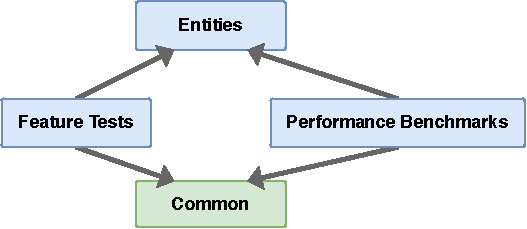
\includegraphics[scale=1]{thesis/img/thesis/01_test_dependencies.drawio.pdf}
  \caption{Test project dependencies.}
  \label{fig:test_project_dependencies}
\end{figure}

Common project is also included. It contains a single class handling loading the database connection string from a configuration file. Dependencies are demonstrated in Figure~\ref{fig:test_project_dependencies}. There is no dependency between feature tests and performance tests. It could be argued that the code for queries could be extracted to a separate class to avoid duplication. But it was kept duplicated to isolate unit tests from performance benchmarks. This structure is repeated for each of the seven examined frameworks.

\subsubsection{Technology overview}
As decided before implementation in Section~\ref{sec:dataset_database}, \acrshort{mssql} with World Wide Importers data set is used. The database system is running in a Docker container. Base image used is \texttt{mssql/server:2022-latest}\footnote{\url{https://hub.docker.com/r/microsoft/mssql-server}} provided by Microsoft. The image imports the dataset and waits until it is ready.

The .NET tests are structured in .NET projects grouped in one solution. .NET version 8 was chosen as it is the latest long term support (\acrshort{lts}) version at the time of writing.\footnote{\url{https://dotnet.microsoft.com/en-us/platform/support/policy/dotnet-core}} Tests are developed and run using Microsoft Visual Studio 2022, but \texttt{dotnet} \acrshort{cli} commands are provided as well.

\subsubsection{Installation instructions}
Source code of unit tests and performance benchmarks, in addition to Dockerfile, are available in a public GitHub repository.\footnote{\url{https://github.com/milan252525/orm-convertor}} The container was tested both in Docker\footnote{\url{https://docs.docker.com/}} and Podman\footnote{\url{https://podman.io/docs}}. A \texttt{Dockerfile} is provided in \texttt{benchmarks/Dockerfile}. Container image can be built and started using the two commands in Listing~\ref{lst:docker_commands}. If needed, \texttt{'docker'} should be replaced by \texttt{'podman'}. The database system will be exposed on port 1444, under username \texttt{'SA'} and password \texttt{'Testingorms123'}.
The third command in Listing~\ref{lst:docker_commands} can be used to test connection. The \texttt{sqlcmd} utility is available only if \acrshort{mssql} is installed locally. Otherwise, any database management tool of choice can be used.

\begin{lstlisting}[language=sh,caption={Command to build, run, and test connection to Docker container.},label={lst:docker_commands}]
docker build -t orm-comparison .

docker run -d --name orm-comparison -p 1444:1433 orm-comparison

sqlcmd -S 127.0.0.1,1444 -U SA -P Testingorms123 -Q "SELECT * FROM [WideWorldImporters].[Purchasing].[PurchaseOrders]"
\end{lstlisting}

To run feature unit tests, build the project in Visual Studio and then use the Test Explorer window to select and run specific tests. Alternatively, navigate to the folder with the solution file and run \lstinline{dotnet test}. This will build the project, find all tests, and run them. 

To run performance benchmarks, set \texttt{BenchmarkMain} as a startup project. Right-click it in the Solution Explorer window and choose \textit{'Set as Startup project'}. Make sure the configuration is set to Release, not Debug. Then start the project without debugging (\texttt{CTRL + F5} keys). A console window will appear. It contains instructions on how to target specific benchmarks. To run all, type in an asterisk (\texttt{'*'}) and press enter. This will trigger a full run, which takes approximately one hour to finish. You can switch to the test configuration which does only a few numbers of iterations in \texttt{BenchmarkMain/Program.cs} file. What the configuration does is further explained in the following sections. 

Console command for running benchmarks is \lstinline{dotnet run --configuration Release --project BenchmarkMain\BenchmarkMain.csproj}. To run with a shorter test configuration, append \lstinline{-- --testb} at the end of the command.

\subsubsection{Feature tests}
For each query defined in Section~\ref{sec:selected_queries}, a unit test in the form of an isolated method is implemented. Connection and other configuration are created outside of the test in a setup part. The method executes the query and correct results are asserted. Assertion checks the amount of results and their order. Each property is tested to contain correct data to ensure mapping was done correctly.

The example below shows Query A1 (see Section~\ref{query:a1}) implemented for Dapper. A single purchase order is retrieved based on its ID, and its properties are checked for correct values. 
\begin{lstlisting}[language=CSharp]
[Fact]
public void A1_EntityIdenticalToTable()
{
    var order = connection.QuerySingle<PurchaseOrder>(
        "SELECT * FROM WideWorldImporters.Purchasing.PurchaseOrders WHERE PurchaseOrderId = @PurchaseOrderId",
        new { PurchaseOrderId = 25 }
    );

    Assert.Multiple(() =>
    {
        Assert.Equal(25, order.PurchaseOrderID);
        Assert.Equal(12, order.SupplierID);
        Assert.Equal(new DateTime(2013, 1, 5), order.OrderDate);
        ...
    });
}
\end{lstlisting}

As decided in Section~\ref{sec:testing_approach}, the \acrshort{linq} query language is used where possible. Otherwise, any available alternative that does not involve just writing raw \acrshort{sql} is preferred. And finally, where nothing else is possible, the raw \acrshort{sql} alternative is selected to have a passing test.  

\subsubsection{Performance benchmarks}
Feature tests can assert the correctness of returned results and overall functionality. But their execution time can greatly vary. There can be some overhead, coming from test initialization or assertions. The system the benchmarks are running on can also impact results.

To solve these problems, BenchmarkDotNet library\footnote{\url{https://benchmarkdotnet.org/}} is used. It allows writing benchmark methods very similar to unit tests. In fact, they are completely identical to unit tests; the only differences are missing assertions and a different method attribute. It allows us to ``transform methods into benchmarks, track their performance, and share reproducible measurement experiments''~\cite{BenchmarkDotNet}. Work with the library is quite easy, it is very configurable and straightforward to run. 

It runs benchmarks for each method multiple times. It starts with a few iterations which will not be included in the results. The first few ensure \textit{just-in-time} (\acrshort{jit}) compilation has taken effect, then multiple iterations without actually running the method code are started to compile overhead. The overhead is removed from the results, ensuring reliability. 

According to BenchmarkDotNet documentation~\cite{BenchmarkDotNetHow}, a single benchmark run consists of the following stages:
\begin{itemize}
    \item \textit{OverheadJitting} -- Measures benchmarking infrastructure compilation.
    \item \textit{WorkloadJitting} -- Measures benchmark method compilation.
    \item \textit{WorkloadPilot} -- Selects best iteration count based on heuristics.
    \item \textit{WorkloadWarmup} -- Runs several iterations before measuring to ensure factors like \acrshort{cpu} caching or branch prediction are optimized.
    \item \textit{WorkloadActual} -- Actual measurements
    \item \textit{WorkloadResult} -- Result calculated from the actual run without the overhead.
\end{itemize}

After the benchmark run finishes, results and run log can be found in folder \path{benchmarks/BenchmarkMain/bin/Release/net8.0/} under a file name \path{BenchmarkDotNet.Artifacts}.

\smallskip
The referenced run results are copied to \path{benchmarks/results/joined}.

\smallskip
Notable result files include:
\begin{itemize}
    \item \path{BenchmarkRun-joined-2025-03-06-16-10-18-report.csv}\\
    Measurements of all benchmarks in \acrshort{csv} format.

    \item \path{BenchmarkRun-joined-2025-03-06-16-10-18-report.html}\\
    Summary table of all benchmarks (\acrshort{html} format).

    \item \path{BenchmarkRun-joined-2025-03-06-16-10-18-report-github.md}\\
    Summary table of all benchmarks (Markdown format suitable for GitHub).

    \item \path{BenchmarkRun-joined-2025-03-06-16-10-18-measurements.csv}\\
    Detailed measurements of every single iteration of each benchmark.
\end{itemize}

\subsection{Interpretation of results}
Results are accompanied by tables showing results across all test cases. 

Table~\ref{tab:feature_comp} summarizes feature test outcomes. The base result indicates if the query could be expressed within each framework (\texttt{'Y'} = yes, \texttt{'N'} = no). Outcomes are categorized as:
\begin{itemize}
    \item \textbf{Y LINQ}: \acrshort{linq} fully supported.
    \item \textbf{Y lambda expr.}: Supported using lambda expressions, less expressive than \acrshort{linq}.
    \item \textbf{Y raw SQL}: Query had to be written directly in \acrshort{sql}, either in string or using a builder.
    \item \textbf{N manually in memory}: Query required manual post-computation in memory.
    \item \textbf{N custom \acrshort{json} parsing/converter}: \acrshort{json} could not be queried and had to be parsed in memory.
    \item \textbf{N error}: Query failed with exception that could not be fixed. 
\end{itemize}
The negative results are discussed in detail further in the subsequent text.

\afterpage{
\begin{landscape}
\begin{table}[htp]
\centering
\caption{Feature comparison results}
\label{tab:feature_comp}
\scriptsize
\begin{threeparttable}[!htb]
\def\arraystretch{1.25}
\begin{tabular}{
>{\raggedright\arraybackslash}p{50.00mm}
>{\raggedright\arraybackslash}p{20.00mm}
>{\raggedright\arraybackslash}p{20.00mm}
>{\raggedright\arraybackslash}p{20.00mm}
>{\raggedright\arraybackslash}p{20.00mm}
>{\raggedright\arraybackslash}p{20.00mm}
>{\raggedright\arraybackslash}p{20.00mm}
>{\raggedright\arraybackslash}p{20.00mm}
>{\raggedright\arraybackslash}p{20.00mm}
}
\toprule
\textbf{Benchmark Name} & \textbf{Dapper} & \textbf{PetaPoco} & \textbf{RepoDB} & \textbf{linq2db} & \textbf{NHibernate} & \textbf{EF6} & \textbf{EF Core} \\
\midrule
A1\_EntityIdenticalToTable &Y raw SQL &Y raw SQL &\cellcolor[HTML]{d9ead3}Y lambda expr. &\cellcolor[HTML]{b7e1cd}Y LINQ &\cellcolor[HTML]{b7e1cd}Y LINQ &\cellcolor[HTML]{b7e1cd}Y LINQ &\cellcolor[HTML]{b7e1cd}Y LINQ \\
A2\_LimitedEntity &Y raw SQL &Y raw SQL &\cellcolor[HTML]{d9ead3}Y lambda expr. &\cellcolor[HTML]{b7e1cd}Y LINQ &\cellcolor[HTML]{b7e1cd}Y LINQ &\cellcolor[HTML]{b7e1cd}Y LINQ &\cellcolor[HTML]{b7e1cd}Y LINQ \\
A3\_MultipleEntitiesFromOneResult &Y raw SQL &Y raw SQL &\cellcolor[HTML]{d9ead3}Y lambda expr. &\cellcolor[HTML]{b7e1cd}Y LINQ &\cellcolor[HTML]{b7e1cd}Y LINQ &\cellcolor[HTML]{b7e1cd}Y LINQ &\cellcolor[HTML]{b7e1cd}Y LINQ \\
A4\_StoredProcedureToEntity &Y raw SQL &Y raw SQL &Y raw SQL &Y raw SQL &\cellcolor[HTML]{ea9999}N error &\cellcolor[HTML]{ea9999}N error &Y raw SQL \\
B1\_SelectionOverIndexedColumn &Y raw SQL &Y raw SQL &\cellcolor[HTML]{d9ead3}Y lambda expr. &\cellcolor[HTML]{b7e1cd}Y LINQ &\cellcolor[HTML]{b7e1cd}Y LINQ &\cellcolor[HTML]{b7e1cd}Y LINQ &\cellcolor[HTML]{b7e1cd}Y LINQ \\
B2\_SelectionOverNonIndexedColumn &Y raw SQL &Y raw SQL &\cellcolor[HTML]{d9ead3}Y lambda expr. &\cellcolor[HTML]{b7e1cd}Y LINQ &\cellcolor[HTML]{b7e1cd}Y LINQ &\cellcolor[HTML]{b7e1cd}Y LINQ &\cellcolor[HTML]{b7e1cd}Y LINQ \\
B3\_RangeQuery &Y raw SQL &Y raw SQL &\cellcolor[HTML]{d9ead3}Y lambda expr. &\cellcolor[HTML]{b7e1cd}Y LINQ &\cellcolor[HTML]{b7e1cd}Y LINQ &\cellcolor[HTML]{b7e1cd}Y LINQ &\cellcolor[HTML]{b7e1cd}Y LINQ \\
B4\_InQuery &Y raw SQL &Y raw SQL &\cellcolor[HTML]{d9ead3}Y lambda expr. &\cellcolor[HTML]{b7e1cd}Y LINQ &\cellcolor[HTML]{b7e1cd}Y LINQ &\cellcolor[HTML]{b7e1cd}Y LINQ &\cellcolor[HTML]{b7e1cd}Y LINQ \\
B5\_TextSearch &Y raw SQL &Y raw SQL &\cellcolor[HTML]{d9ead3}Y lambda expr. &\cellcolor[HTML]{b7e1cd}Y LINQ &\cellcolor[HTML]{b7e1cd}Y LINQ &\cellcolor[HTML]{b7e1cd}Y LINQ &\cellcolor[HTML]{b7e1cd}Y LINQ \\
B6\_PagingQuery &Y raw SQL &Y raw SQL &\cellcolor[HTML]{d9ead3}Y lambda expr. &\cellcolor[HTML]{b7e1cd}Y LINQ &\cellcolor[HTML]{b7e1cd}Y LINQ &\cellcolor[HTML]{b7e1cd}Y LINQ &\cellcolor[HTML]{b7e1cd}Y LINQ \\
C1\_AggregationCount &Y raw SQL &Y raw SQL &\cellcolor[HTML]{f4cccc}N manually in memory &\cellcolor[HTML]{b7e1cd}Y LINQ &\cellcolor[HTML]{b7e1cd}Y LINQ &\cellcolor[HTML]{b7e1cd}Y LINQ &\cellcolor[HTML]{b7e1cd}Y LINQ \\
C2\_AggregationMax &Y raw SQL &Y raw SQL &\cellcolor[HTML]{d9ead3}Y lambda expr. &\cellcolor[HTML]{b7e1cd}Y LINQ &\cellcolor[HTML]{b7e1cd}Y LINQ &\cellcolor[HTML]{b7e1cd}Y LINQ &\cellcolor[HTML]{b7e1cd}Y LINQ \\
C3\_AggregationSum &Y raw SQL &Y raw SQL &Y raw SQL &\cellcolor[HTML]{b7e1cd}Y LINQ &\cellcolor[HTML]{b7e1cd}Y LINQ &\cellcolor[HTML]{b7e1cd}Y LINQ &\cellcolor[HTML]{b7e1cd}Y LINQ \\
D1\_OneToManyRelationship &\cellcolor[HTML]{f4cccc}N manually in memory &\cellcolor[HTML]{f4cccc}N manually in memory &\cellcolor[HTML]{d9ead3}Y lambda expr. &\cellcolor[HTML]{b7e1cd}Y LINQ + mapping &\cellcolor[HTML]{b7e1cd}Y LINQ + mapping &\cellcolor[HTML]{b7e1cd}Y LINQ + mapping &\cellcolor[HTML]{b7e1cd}Y LINQ + mapping \\
D2\_ManyToManyRelationship &\cellcolor[HTML]{f4cccc}N manually in memory &\cellcolor[HTML]{f4cccc}N manually in memory &\cellcolor[HTML]{f4cccc}N manually in memory &\cellcolor[HTML]{b7e1cd}Y LINQ + mapping, join entity &\cellcolor[HTML]{b7e1cd}Y LINQ + mapping &\cellcolor[HTML]{b7e1cd}Y LINQ + mapping &\cellcolor[HTML]{b7e1cd}Y LINQ + mapping \\
D3\_OptionalRelationship &\cellcolor[HTML]{f4cccc}N manually in memory &\cellcolor[HTML]{f4cccc}N manually in memory &\cellcolor[HTML]{d9ead3}Y lambda expr. &\cellcolor[HTML]{b7e1cd}Y LINQ + mapping &\cellcolor[HTML]{b7e1cd}Y LINQ + mapping &\cellcolor[HTML]{b7e1cd}Y LINQ + mapping &\cellcolor[HTML]{b7e1cd}Y LINQ + mapping \\
E1\_ColumnSorting &Y raw SQL &Y raw SQL &\cellcolor[HTML]{d9ead3}Y lambda expr. &\cellcolor[HTML]{b7e1cd}Y LINQ &\cellcolor[HTML]{b7e1cd}Y LINQ &\cellcolor[HTML]{b7e1cd}Y LINQ &\cellcolor[HTML]{b7e1cd}Y LINQ \\
E2\_Distinct &Y raw SQL &Y raw SQL &Y raw SQL &\cellcolor[HTML]{b7e1cd}Y LINQ &\cellcolor[HTML]{b7e1cd}Y LINQ &\cellcolor[HTML]{b7e1cd}Y LINQ &\cellcolor[HTML]{b7e1cd}Y LINQ \\
F1\_NestedJSONQuery &\cellcolor[HTML]{f4cccc}N custom JSON parsing &\cellcolor[HTML]{f4cccc}N custom JSON parsing &\cellcolor[HTML]{f4cccc}N custom JSON parsing &\cellcolor[HTML]{f4cccc}N custom converter &\cellcolor[HTML]{f4cccc}N custom JSON parsing &\cellcolor[HTML]{f4cccc}N custom JSON parsing &\cellcolor[HTML]{b7e1cd}Y LINQ \\
F2\_JSONArrayQuery &\cellcolor[HTML]{f4cccc}N custom JSON parsing &\cellcolor[HTML]{f4cccc}N custom JSON parsing &\cellcolor[HTML]{f4cccc}N custom JSON parsing &\cellcolor[HTML]{f4cccc}N custom converter &\cellcolor[HTML]{f4cccc}N custom JSON parsing &\cellcolor[HTML]{f4cccc}N custom JSON parsing &\cellcolor[HTML]{b7e1cd}Y LINQ \\
G1\_Union &Y raw SQL &Y raw SQL &Y raw SQL &\cellcolor[HTML]{b7e1cd}Y LINQ &\cellcolor[HTML]{b7e1cd}Y LINQ &\cellcolor[HTML]{b7e1cd}Y LINQ &\cellcolor[HTML]{b7e1cd}Y LINQ \\
G2\_Intersection &Y raw SQL &Y raw SQL &Y raw SQL &\cellcolor[HTML]{b7e1cd}Y LINQ &\cellcolor[HTML]{b7e1cd}Y LINQ &\cellcolor[HTML]{b7e1cd}Y LINQ &\cellcolor[HTML]{b7e1cd}Y LINQ \\
H1\_Metadata &Y raw SQL &Y raw SQL &Y raw SQL &Y raw SQL &Y raw SQL &Y raw SQL &Y raw SQL \\
\bottomrule
\end{tabular}
\end{threeparttable}
\end{table}
\end{landscape}
}

Table~\ref{tab:benchmark_results_time} presents measured execution time (in microseconds), and Table~\ref{tab:benchmark_results_memory} presents allocated memory during the run of the benchmark. Reported numbers in text are rounded to the nearest integer.

Performance tests have to be considered in the context of the feature test results. It was not possible to write all tests in the same way across all frameworks. In some cases, pure ADO.NET queries were used when the framework failed entirely. Additionally, some queries required additional processing in memory, significantly affecting memory usage. These anomalies are explicitly noted.

Certain frameworks cannot log generated \acrshort{sql} statements to console or file. For those, Microsoft SQL Server Profiler\footnote{\url{https://learn.microsoft.com/en-us/sql/tools/sql-server-profiler/sql-server-profiler}} is used. It allows capturing of any event happening in the \acrshort{mssql} database, including incoming \acrshort{sql} queries. That allows inspection of the raw query after it leaves the application as the frameworks can make no further edits to it.

\afterpage{
\begin{landscape}
\begin{table}
\centering
\caption{Performance benchmark results - Mean time (\unit{\micro\second})}
\label{tab:benchmark_results_time}
\scriptsize
\def\arraystretch{1.50}
\begin{tabular}{
>{\raggedright\arraybackslash}p{50.00mm}
>{\raggedleft\arraybackslash}p{20.00mm}
>{\raggedleft\arraybackslash}p{20.00mm}
>{\raggedleft\arraybackslash}p{20.00mm}
>{\raggedleft\arraybackslash}p{20.00mm}
>{\raggedleft\arraybackslash}p{20.00mm}
>{\raggedleft\arraybackslash}p{20.00mm}
>{\raggedleft\arraybackslash}p{20.00mm}
>{\raggedleft\arraybackslash}p{20.00mm}
}
\toprule
\textbf{Namespace} &    \textbf{Dapper} &  \textbf{PetaPoco} &    \textbf{RepoDB} &   \textbf{Linq2db} &  \textbf{NHibernate} &        \textbf{EF6} &     \textbf{EFCore} \\
\midrule
A1\_EntityIdenticalToTable        &      750 &     \cellcolor[HTML]{b7e1cd} 722 &      748 &      839 &        742 &        \cellcolor[HTML]{f4cccc} 854 &        809 \\
A2\_LimitedEntity                 &     \cellcolor[HTML]{b7e1cd} 718 &      726 &      735 &      858 &       \cellcolor[HTML]{f4cccc} 958 &        882 &        799 \\
A3\_MultipleEntitiesFromOneResult &     \cellcolor[HTML]{b7e1cd} 736 &      \cellcolor[HTML]{b7e1cd}736 &      745 &      898 &     \cellcolor[HTML]{f4cccc} 1 001 &        945 &        832 \\
A4\_StoredProcedureToEntity       &  523 239 & \cellcolor[HTML]{b7e1cd} 505 967 &  523 242 &  519 491 &   \cellcolor[HTML]{f4cccc} 621 739 &    514 077 &    521 573 \\
B1\_SelectionOverIndexedColumn    &     \cellcolor[HTML]{b7e1cd} 744 &      759 &      762 &      868 &        817 &       \cellcolor[HTML]{f4cccc} 905 &        806 \\
B2\_SelectionOverNonIndexedColumn &   43 612 &  \cellcolor[HTML]{b7e1cd} 41 100 &   43 052 &   43 708 &     86 419 &   \cellcolor[HTML]{f4cccc} 125 169 &     48 016 \\
B3\_RangeQuery                    &   30 393 &   29 935 &  \cellcolor[HTML]{f4cccc} 30 746 &   21 909 &     22 289 &     22 823 &    \cellcolor[HTML]{b7e1cd} 21 102 \\
B4\_InQuery                       &      856 &     \cellcolor[HTML]{b7e1cd} 855 &      876 &      954 &        945 &     \cellcolor[HTML]{f4cccc} 1 408 &      1 147 \\
B5\_TextSearch                    & \cellcolor[HTML]{f4cccc} 747 728 &  747 721 &  745 551 &  745 319 &    746 464 &    746 264 &   \cellcolor[HTML]{b7e1cd} 744 754 \\
B6\_PagingQuery                   &    1 327 &   \cellcolor[HTML]{b7e1cd} 1 314 &    1 556 &    1 458 &      1 447 &     \cellcolor[HTML]{f4cccc} 1 710 &      1 406 \\
C1\_AggregationCount              &  \cellcolor[HTML]{b7e1cd} 35 006 &   35 289 & \cellcolor[HTML]{f4cccc} 377 349 &   35 372 &     35 553 &     35 364 &     35 286 \\
C2\_AggregationMax                &    1 240 &  \cellcolor[HTML]{b7e1cd}  1 227 &    1 264 &   \cellcolor[HTML]{f4cccc} 1 380 &      1 291 &      1 366 &      1 304 \\
C3\_AggregationSum                &   86 499 &   85 944 &   86 899 &   86 145 &     75 137 &    \cellcolor[HTML]{b7e1cd} 69 827 &    \cellcolor[HTML]{f4cccc} 87 825 \\
D1\_OneToManyRelationship         &      781 &     \cellcolor[HTML]{b7e1cd} 770 &      806 &   \cellcolor[HTML]{f4cccc} 2 997 &      1 042 &      1 581 &        895 \\
D2\_ManyToManyRelationship        &    4 584 &  \cellcolor[HTML]{b7e1cd}  4 480 &    6 031 &    9 383 &      5 940 &      6 913 &    \cellcolor[HTML]{f4cccc} 14 964 \\
D3\_OptionalRelationship          &  187 693 &  172 030 &  393 631 &  \cellcolor[HTML]{b7e1cd} 91 326 &    533 489 &  1 993 146 & \cellcolor[HTML]{f4cccc} 2 548 411 \\
E1\_ColumnSorting                 &    4 725 &   \cellcolor[HTML]{b7e1cd} 4 622 &    4 963 &    4 845 &     \cellcolor[HTML]{f4cccc} 6 316 &      6 204 &      4 885 \\
E2\_Distinct                      &    2 181 &  \cellcolor[HTML]{b7e1cd}  2 148 &    2 180 &   \cellcolor[HTML]{f4cccc} 2 374 &      2 229 &      2 340 &      2 270 \\
F1\_JSONObjectQuery               &    1 459 &    1 478 &  \cellcolor[HTML]{b7e1cd}  1 457 &   \cellcolor[HTML]{f4cccc} 1 552 &      1 494 &      1 490 &      1 544 \\
F2\_JSONArrayQuery                &    1 723 &   \cellcolor[HTML]{b7e1cd} 1 718 &    1 732 &    1 795 &      1 761 &      1 771 &     \cellcolor[HTML]{f4cccc} 1 839 \\
G1\_Union                         &      728 &    \cellcolor[HTML]{b7e1cd}  715 &      723 &    1 580 &      1 538 &     \cellcolor[HTML]{f4cccc} 1 613 &      1 561 \\
G2\_Intersection                  &      739 &     \cellcolor[HTML]{b7e1cd} 718 &      730 &    1 596 &      1 534 &     \cellcolor[HTML]{f4cccc} 1 622 &      1 566 \\
H1\_Metadata                      &      851 &      843 &      844 &     \cellcolor[HTML]{f4cccc} 925 &        866 &        899 &      \cellcolor[HTML]{b7e1cd}  814 \\
\bottomrule
\end{tabular}
\end{table}
\end{landscape}
}

\afterpage{
\begin{landscape}
\begin{table}
\centering
\caption{Performance benchmark results - Allocated memory (KB)}
\label{tab:benchmark_results_memory}
\scriptsize
\def\arraystretch{1.50}
\begin{tabular}{
>{\raggedright\arraybackslash}p{50.00mm}
>{\raggedleft\arraybackslash}p{20.00mm}
>{\raggedleft\arraybackslash}p{20.00mm}
>{\raggedleft\arraybackslash}p{20.00mm}
>{\raggedleft\arraybackslash}p{20.00mm}
>{\raggedleft\arraybackslash}p{20.00mm}
>{\raggedleft\arraybackslash}p{20.00mm}
>{\raggedleft\arraybackslash}p{20.00mm}
>{\raggedleft\arraybackslash}p{20.00mm}
}
\toprule
\textbf{Namespace}                         &    \textbf{Dapper} &  \textbf{PetaPoco} &    \textbf{RepoDB} &   \textbf{Linq2db} & \textbf{NHibernate} &      \textbf{EF6} &    \textbf{EFCore} \\
\midrule
A1\_EntityIdenticalToTable        &    \cellcolor[HTML]{b7e1cd}  6.24 &     7.99 &      8.77 &     12.74 &      36.06 &   \cellcolor[HTML]{f4cccc} 90.43 &    14.49 \\
A2\_LimitedEntity                 &    \cellcolor[HTML]{b7e1cd}  4.74 &     9.64 &      7.99 &     18.25 &      50.70 &  \cellcolor[HTML]{f4cccc} 115.18 &    16.11 \\
A3\_MultipleEntitiesFromOneResult &    \cellcolor[HTML]{b7e1cd}  7.28 &    13.03 &     10.38 &     27.74 &      84.00 &  \cellcolor[HTML]{f4cccc} 211.61 &    25.85 \\
A4\_StoredProcedureToEntity       &  24 294.84 & \cellcolor[HTML]{b7e1cd}16 490.15 &  17 007.14 &  16 490.93 &  \cellcolor[HTML]{f4cccc} 91 569.96 & 35 270.68 & 29 008.69 \\
B1\_SelectionOverIndexedColumn    &    \cellcolor[HTML]{b7e1cd}  8.63 &    14.30 &      9.79 &     14.63 &      49.46 &  \cellcolor[HTML]{f4cccc} 102.35 &    12.88 \\
B2\_SelectionOverNonIndexedColumn &   7 112.75 & \cellcolor[HTML]{b7e1cd} 3 308.54 &   3 410.07 &   3 314.16 &   21 371.02 & \cellcolor[HTML]{f4cccc} 50 014.45 &  5 847.86 \\
B3\_RangeQuery                    &    989.93 &  \cellcolor[HTML]{b7e1cd} 468.38 &    480.34 &    475.55 &    3 048.82 & \cellcolor[HTML]{f4cccc} 6 747.98 &   819.92 \\
B4\_InQuery                       &     16.92 &    20.34 &    \cellcolor[HTML]{b7e1cd} 16.64 &     19.58 &      87.42 &  \cellcolor[HTML]{f4cccc} 354.18 &    19.85 \\
B5\_TextSearch                    &   1 169.29 &  \cellcolor[HTML]{b7e1cd} 587.24 &    599.41 &    592.78 &    3 472.99 & \cellcolor[HTML]{f4cccc} 8 113.77 &   979.42 \\
B6\_PagingQuery                   &     32.59 &    25.06 &    \cellcolor[HTML]{b7e1cd} 18.25 &     26.58 &     128.29 &  \cellcolor[HTML]{f4cccc} 265.26 &    40.52 \\
C1\_AggregationCount              &    \cellcolor[HTML]{b7e1cd}  2.75 &     8.79 & \cellcolor[HTML]{f4cccc} 59 994.30 &     12.46 &      41.75 &   117.99 &    12.04 \\
C2\_AggregationMax                &      1.97 &     4.19 &     \cellcolor[HTML]{b7e1cd} 1.77 &      8.12 &      23.06 &   \cellcolor[HTML]{f4cccc} 77.09 &     5.69 \\
C3\_AggregationSum                &      2.09 &     4.41 &     \cellcolor[HTML]{b7e1cd} 1.35 &      9.25 &      25.31 &   \cellcolor[HTML]{f4cccc} 81.72 &     6.85 \\
D1\_OneToManyRelationship         &   \cellcolor[HTML]{b7e1cd}  16.46 &    17.94 &     20.23 &     24.58 &      88.71 &  \cellcolor[HTML]{f4cccc} 115.27 &    26.44 \\
D2\_ManyToManyRelationship        &    433.35 &  \cellcolor[HTML]{b7e1cd} 381.13 &    854.28 &    352.15 &    1 162.43 &  1 395.95 & \cellcolor[HTML]{f4cccc} 2 555.79 \\
D3\_OptionalRelationship          &  40 923.17 & 24 909.64 &  20 945.39 &  \cellcolor[HTML]{b7e1cd} 9 083.71 &  144 094.98 &\cellcolor[HTML]{f4cccc}278 566.55 &175 866.23 \\
E1\_ColumnSorting                 &    349.40 &  \cellcolor[HTML]{b7e1cd} 156.96 &    162.62 &    162.54 &    1 354.02 & \cellcolor[HTML]{f4cccc} 2 000.95 &   348.07 \\
E2\_Distinct                      &      2.42 &     4.78 &    \cellcolor[HTML]{b7e1cd}  1.66 &      9.34 &      23.72 &   \cellcolor[HTML]{f4cccc} 76.19 &     8.54 \\
F1\_JSONObjectQuery               &   \cellcolor[HTML]{b7e1cd}  21.71 &    45.25 &     31.82 &     27.09 &     \cellcolor[HTML]{f4cccc} 86.13 &    73.38 &    51.68 \\
F2\_JSONArrayQuery                &    \cellcolor[HTML]{b7e1cd}  6.04 &    18.12 &      8.25 &     11.30 &     \cellcolor[HTML]{f4cccc} 74.31 &    57.24 &    16.86 \\
G1\_Union                         &      2.39 &     3.45 &    \cellcolor[HTML]{b7e1cd}  1.40 &     18.03 &      60.07 &  \cellcolor[HTML]{f4cccc} 136.10 &    20.35 \\
G2\_Intersection                  &      2.17 &     3.25 &     \cellcolor[HTML]{b7e1cd} 1.30 &     17.91 &      61.36 &  \cellcolor[HTML]{f4cccc} 135.98 &    21.73 \\
H1\_Metadata                      &      1.98 &     5.10 &    \cellcolor[HTML]{b7e1cd}  1.21 &      5.61 &      35.53 &   \cellcolor[HTML]{f4cccc} 46.52 &    10.99 \\
\bottomrule
\end{tabular}
\end{table}
\end{landscape}
}

\subsubsection{Benchmark execution environment}
Performance benchmarks were executed on a single computer configured for the highest performance:
\begin{itemize}
    \item Windows 11, AMD Ryzen 5 5600H \acrshort{cpu} (6 physical cores, 12 logical)
    \item .NET \acrshort{sdk} version: 9.0.101
    \item Execution framework: BenchmarkDotNet v0.14.0
    \item Runtime: .NET 8.0.11, X64 architecture, RyuJIT AVX2
\end{itemize}

\subsubsection{Group A -- Entity projection}
The first three queries, i.e., \hyperref[query:a1]{A1}, \hyperref[query:a2]{A2}, and \hyperref[query:a3]{A3}, fetched and reshaped one database record successfully across all frameworks. Macro \acrshort{orm}(s), i.e., \acrshort{ef}, and NHibernate, used \acrshort{linq} \texttt{Select} method. Micro \acrshort{orm}(s) utilized projection in \acrshort{sql} query directly.
Minor performance differences appeared, macro \acrshort{orm}(s) were slightly slower. Notably, NHibernate and \acrshort{ef}6 showed significant 2 to 10 times memory allocation spikes. \acrshort{ef} Core is clearly optimized in this area.

Query~\hyperref[query:a4]{A4} tested loading results of a stored procedure. The volume of data is approximately 60,000 rows. The stored procedure in our test dataset returns column names with spaces. Which is definitely unusual, but we would not expect a framework to completely fail. Dapper, PetaPoco, RepoDB, linq2db, and \acrshort{ef} Core succeeded using raw \acrshort{sql}. Memory allocation varied significantly for those (16 MB to 29 MB). No major difference in the executed query was found using SQL Server Profiler.

NHibernate failed on an internal error. The error message \textit{Could not find a setter for property 'WWI Order ID' in class 'System.RuntimeType'} suggests the framework failed to fill an internal memory representation of the entity. A workaround using a hash table increased both time and memory significantly.

\acrshort{ef}6 completely failed, with no viable workaround this time. The test uses a pure ADO.NET connection, with no \acrshort{ef}6 features whatsoever. We consider the test failed, and the measurements are not relevant for our comparison.

\subsubsection{Group B -- Selection}
All selection queries \hyperref[query:b1]{B1} -- \hyperref[query:b6]{B6} passed in terms of features. As expected, Dapper and PetaPoco required explicit \acrshort{sql}, while macro \acrshort{orm}(s) supported \acrshort{linq}. Memory usage varied significantly, particularly for NHibernate and \acrshort{ef}6.

Query \hyperref[query:b1]{B1}, which returns 5 records, showed macro \acrshort{orm}(s) allocating significantly more memory (NHibernate 49 KB, \acrshort{ef}6 102 KB) compared to Dapper (9 KB) or PetaPoco (14 KB). Query \hyperref[query:b2]{B2}, returning thousands of records, again showed NHibernate and \acrshort{ef}6 taking drastically more time and memory (7 and 16 times more), even though generated \acrshort{sql} queries were identical.

Query \hyperref[query:b3]{B3} showed unexpectedly slower performance from Dapper, PetaPoco, and RepoDB. There is a difference in the query. In Dapper and PetaPoco, where \acrshort{sql} is written by us, we used \texttt{BETWEEN} condition for selecting a date range. Other \acrshort{orm}(s) broke this condition down into two operators ($\leq$ and $\geq$). But RepoDB does not use \texttt{BETWEEN}, hinting that the difference had no impact on performance.

Queries \hyperref[query:b4]{B4}, \hyperref[query:b5]{B5}, and \hyperref[query:b6]{B6} had generally consistent execution times across all frameworks. But NHibernate and \acrshort{ef}6 showed consistently elevated memory allocation. Interestingly, in some cases, Dapper showed higher memory usage compared to PetaPoco, indicating differences in internal memory optimization. 

\subsubsection{Group C -- Aggregation}
Aggregation tests \hyperref[query:c1]{C1} -- \hyperref[query:c3]{C3} tested handling of groupings and aggregate functions. RepoDB lacked support for \texttt{GROUP BY} operation in query \hyperref[query:c1]{C1}, failing the test entirely. NHibernate and \acrshort{ef}6 have approximately 4 and 10 times memory consumption increase, respectively, although execution times remain comparable. 

\hyperref[query:c2]{C2} showed consistent performance and memory usage across frameworks. However, in \hyperref[query:c3]{C3}, RepoDB incorrectly handled a multiplication when using its \texttt{Sum} function. It omitted part of the multiplication inside the \texttt{Sum} aggregation function, returning incorrect results. A raw \acrshort{sql} query had to be used instead. The measured time is consistent across all frameworks. The returned result is just one number and we can see some slight increase in memory consumption for the macro \acrshort{orm}(s).

In summary, RepoDB did not handle aggregation functions well. \acrshort{ef} Core is showing its optimization by approaching the results of micro \acrshort{orm}(s).

\subsubsection{Group D -- Relations}
This group evaluates how effectively \acrshort{orm}(s) handle relational data -- specifically one-to-many, many-to-many, and optional one-to-many relationships. Macro \acrshort{orm}(s) managed to automatically retrieve related entities once mapping was correctly defined. On the other hand, micro \acrshort{orm}(s) generally required raw \acrshort{sql} data fetching and in-memory grouping. Parent-child pairs were fetched individually before grouping them using dictionaries.

In query \hyperref[query:d1]{D1}, one parent with a few children was fetched. NHibernate and \acrshort{ef}6 again showed increased memory usage, around 4 to 6 times higher.

Query \hyperref[query:d2]{D2} examined a dense many-to-many relationship involving 227 entities on one side and 10 on the other. RepoDB passed the other two queries, but this one had to be done in memory. Linq2db required an explicit join entity, while the other macro \acrshort{orm}(s) directly mapped child collections within parent entities.

Query \hyperref[query:d3]{D3} tested an optional one-to-many relationship. Linq2db had the best results, using separate queries for parents and children without any optimization enabled. Surprisingly, \acrshort{ef} Core performed the worst, taking 2548 ms compared to Dapper's 187 ms. This inefficiency remained even after experimenting with different tracking settings and the split query feature. When running the raw generated query directly, it was executed in less than 200 ms.

We could see \acrshort{ef} Core performing well among the previous categories, but it is really slow when it comes to relationships. Raw \acrshort{sql} combined with manual memory grouping or using linq2db seems to be the best option for queries over relationships.

\subsubsection{Group E -- Result modification}
Queries \hyperref[query:e1]{E1} and \hyperref[query:e2]{E2} tested column sorting and distinct results. All \acrshort{orm}(s) passed these tests with no significant difference. Only NHibernate and \acrshort{ef}6 showed increased memory consumption. 

\subsubsection{Group F -- Querying JSON}
These tests targeted \acrshort{json} querying capabilities within a string column. Only \acrshort{ef} Core provides full \acrshort{linq} integration. Other frameworks required raw \acrshort{sql} with \acrshort{mssql} \acrshort{json} functions and subsequent manual \acrshort{json} parsing.

Both queries \hyperref[query:f1]{F1} and \hyperref[query:f2]{F2} showed similar execution times. Allocated memory differs slightly, mainly for NHibernate and \acrshort{ef}6 once again. Interestingly, PetaPoco consumed over twice the memory of Dapper despite identical queries.

\subsubsection{Group G -- Set operations}
Query \hyperref[query:g1]{G1} tested union and \hyperref[query:g2]{G2} intersection. Macro \acrshort{orm}(s) took roughly double the time. However, considering the small result set ($<$ 10), the variation can likely be attributed to framework overhead.

\subsubsection{Group H -- Querying metadata}
The final test \hyperref[query:h1]{H1} queried table metadata, specifically the data type of a single column. No \acrshort{orm} had native support, requiring a raw \acrshort{sql} query to \texttt{INFORMATION\_SCHEMA.COLUMNS} table. There are small differences, we can likely attribute them to framework overhead.

\subsubsection{Summary of findings}
Performance and feature test results clearly differ between micro and macro \acrshort{orm}(s). Macro \acrshort{orm}(s) (i.e., NHibernate, \acrshort{ef}6, \acrshort{ef} Core) offer richer features and better abstractions. But that comes at the cost of increased execution time and memory overhead, particularly noticeable in the older \acrshort{ef}6 and NHibernate. \acrshort{ef} Core consistently demonstrates strong optimizations, often competing with micro \acrshort{orm}(s). However, it notably struggles with relational queries. 

Micro \acrshort{orm}(s) (i.e., Dapper and PetaPoco) require manual \acrshort{sql} handling, resulting in minimal time and memory overhead. They generally handle their limited features well. Linq2db strikes a good balance between speed and abstraction over \acrshort{sql}. It handles complex relationships notably well. Lastly, RepoDB stands at a strange middle ground, neither being best in any category nor offering a wide range of features.

Considering our test results alongside other factors -- our previous findings about popularity, update frequency and overall functionality -- \acrshort{ef} Core emerges as the best choice for most applications. It has the widest feature set with solid optimizations. However, when performance is the critical factor, choosing raw queries with Dapper might be a better alternative.





